% !TEX TS-program = xelatex
\documentclass[12pt,letterpaper]{article}

% ===========================
% HOUSE STYLE PREAMBLE
% ===========================
\usepackage{fontspec}

\setmainfont{EB Garamond}[
  Numbers=OldStyle,
  Ligatures=TeX,
]

% IPA fallback font
\newfontfamily\ipafont{Charis SIL}
\newcommand{\ipa}[1]{{\ipafont #1}}

% Lining figures when needed (tables, years in isolation)
\providecommand{\liningnums}[1]{{\addfontfeatures{Numbers=Lining}#1}}

% Monospace
\setmonofont{Inconsolata}[Scale=MatchLowercase]

% ===========================
% PAGE LAYOUT
% ===========================
\usepackage[
  letterpaper,
  inner=1.25in,
  outer=1in,
  top=1in,
  bottom=1.25in,
  marginparwidth=0.6in,
]{geometry}

\usepackage[british]{babel}
\usepackage[final]{microtype}

% ===========================
% HEADINGS
% ===========================
\usepackage{titlesec}

% Section: small caps, number in margin
\titleformat{\section}
  {\normalfont\scshape}
  {\llap{\thesection\quad}}
  {0pt}
  {}

% Subsection: small caps sentence case
\titleformat{\subsection}
  {\normalfont\scshape}
  {\thesubsection\quad}
  {0pt}
  {}

% Subsubsection: upright
\titleformat{\subsubsection}
  {\normalfont}
  {\thesubsubsection\quad}
  {0pt}
  {}

% Spacing
\titlespacing*{\section}{0pt}{2ex plus 1ex minus .2ex}{1ex plus .2ex}
\titlespacing*{\subsection}{0pt}{1.5ex plus 1ex minus .2ex}{0.5ex plus .2ex}
\titlespacing*{\subsubsection}{0pt}{1ex plus 0.5ex minus .1ex}{0.3ex plus .1ex}

% ===========================
% RUNNING HEADS
% ===========================
\usepackage{fancyhdr}
\pagestyle{fancy}
\fancyhf{}
\fancyhead[L]{\small\scshape\leftmark}
\fancyhead[R]{\small\thepage}
\fancyfoot{}
\setlength{\headheight}{13.6pt}
\addtolength{\topmargin}{-1.6pt}
\renewcommand{\headrulewidth}{0pt}

% ===========================
% COLORS & HYPERLINKS
% ===========================
\usepackage{xcolor}
\definecolor{linkmaroon}{RGB}{128, 0, 32}

\usepackage{hyperref}
\hypersetup{
    colorlinks=true,
    linkcolor=linkmaroon,
    filecolor=linkmaroon,
    citecolor=linkmaroon,    
    urlcolor=linkmaroon,
    pdftitle={Grammaticality de-idealized},
    pdfauthor={Brett Reynolds},
}
\usepackage{orcidlink}

% ===========================
% QUOTATIONS
% ===========================
\usepackage[style=american]{csquotes} 
\MakeOuterQuote{"}

% ===========================
% SEMANTIC MACROS
% ===========================
\newcommand{\term}[1]{\textsc{#1}}
\newcommand{\mention}[1]{\textit{#1}}
\newcommand{\mentionh}[1]{⟨#1⟩}
\newcommand{\olang}[1]{\textit{#1}}
\newcommand{\abbr}[1]{\textsc{#1}}
\usepackage{marvosym}
\newcommand{\crossmark}{\textsubscript{\Cross}}

% ===========================
% MATHS AND SYMBOLS
% ===========================
\usepackage{amsmath,amssymb}

% ===========================
% LINGUISTIC EXAMPLES
% ===========================


% Judgement markers (TEXT-MODE SAFE)
\newcommand{\judgesep}{\kern-0.15em}
\newcommand{\ungram}[1]{*\judgesep#1}
\newcommand{\marg}[1]{?\judgesep#1}
\newcommand{\odd}[1]{\#\judgesep#1}

% ===========================
% LISTS
% ===========================
\usepackage{enumitem}
\setlist{nosep, leftmargin=*}
\setlist[enumerate]{label=\arabic*.}
\setlist[itemize]{label=--}

% ===========================
% TABLES & FIGURES
% ===========================
\usepackage{booktabs}
\usepackage{array}
\usepackage{graphicx}
\graphicspath{{figures/}}

% ===========================
% BIBLIOGRAPHY
% ===========================
\usepackage[backend=biber,style=apa,natbib=true,doi=true,isbn=false,url=true]{biblatex}
\addbibresource{refs.bib}

% Possessive citation
\newcommand{\posscite}[1]{\citeauthor{#1}'s (\citeyear{#1})}

% ===========================
% UTILITIES
% ===========================
\usepackage{xspace}
\newcommand{\eg}{e.g.\,\xspace}
\newcommand{\ie}{i.e.\,\xspace}
\newcommand{\etc}{etc.\xspace}

% ===========================
% DOCUMENT SPECIFIC PACKAGES
% ===========================
% Required for simulation plots and notes
\usepackage{pgfplots}
\pgfplotsset{compat=1.18}
\usepackage{tikz}
\usetikzlibrary{arrows.meta,shapes,positioning,fit,backgrounds}
\usepackage[most]{tcolorbox}
\definecolor{lsLightGray}{RGB}{240,240,240}
\definecolor{lsMidBlue}{RGB}{0,114,178}
\newtcolorbox{note}{
  colback=lsLightGray,
  colframe=lsMidBlue,
  boxrule=0.5pt,
  sharp corners,
}
\usepackage{rotating}

% ===========================
% LINGUISTIC EXAMPLES (Must be last)
% ===========================
\usepackage{langsci-gb4e}
\makeatletter
\@ifundefined{noautomath}{}{\noautomath}
\makeatother

\title{Grammaticality de-idealized}
\author{Brett Reynolds \orcidlink{0000-0003-0073-7195}\\
  Humber Polytechnic \& University of Toronto\\
  \href{mailto:brett.reynolds@humber.ca}{brett.reynolds@humber.ca}}
\date{\today}

\begin{document}
\maketitle

\begin{abstract}
    This paper introduces a novel theoretical framework for (un)gram\-maticality, distinct from traditional grammars focused solely on language production or description. The proposed model conceptualizes (un)grammaticality explicitly as coherence in conditioned form--value relations accepted or rejected by language communities, integrating morphosyntactic, semantic--pragmatic, and social dimensions. Previous approaches, including generative grammar, Construction Grammar, and psycholinguistic models, haven't adequately explained why grammaticality is specifically restricted to morphosyntax, why semantically coherent constructions may nonetheless be deemed ungrammatical, or why certain semantically transparent structures remain systematically blocked. The present framework addresses these gaps by providing a principled explanation of (un)grammaticality rooted in community standards for communicative coherence, rather than relying exclusively on structural or intuition-based definitions.
\end{abstract}

%\url{https://chatgpt.com/share/68498638-5d38-8009-94ca-7007915fe08a}

\newpage
\section*{Introduction}

Every competent speaker of English knows that \ungram{\mention{Can the have running}} is impossible, but the source of this certainty proves remarkably elusive. What does it mean to say a sentence is ungrammatical? Consider these examples:

\ea \label{ex:starting-stars}
\ea\label{ex:nonsense} \ungram{\mention{Can the have running?}}
\ex\label{ex:colorless-grammatica} \mention{Colorless green ideas sleep furiously.} \autocite{chomsky1957}
\ex\label{ex:tense} \ungram{\mention{I've finished it yesterday.}}
\ex\marg{\mention{I saw Joan, a friend of whose was visiting.}}\label{ex:whose} 
\ex\label{ex:center} \mention{The bread the baker the apprentice helped made is delicious.}
\ex\label{ex:age} \textbf{A:} \mention{How old are you?} \textbf{B:} \ungram{\mention{I have 25 years.}}
\ex\label{ex:lbe} \ungram{\mention{Which did you buy car?}}
\z\z

While all might receive asterisks in many analyses, they represent fundamentally different types of unacceptability. Some constructions, like (\ref{ex:nonsense}), fail to pair form with any meaning in English. Others, like (\ref{ex:tense}), involve a clash between the time semantics of clause tense and the word \textit{yesterday}. Still others, such as (\ref{ex:whose}) show gradient or indeterminate status. (\ref{ex:center}) illustrates what might be called theoretically predicted acceptability~-- constructions that linguistic theory predicts should be grammatical but are consistently rejected by native speakers. Still others, like (\ref{ex:age}) are grammatical in some contexts but not others. And a few, like the left-branch extraction of (\ref{ex:lbe}), seem to be ruled out entirely, despite being apparently short and interpretable.

Different theoretical traditions have emphasized different aspects of grammaticality: formal approaches focus on abstract principles, usage-based theories stress frequency and entrenchment, and processing accounts highlight cognitive constraints. But the field still lacks a unified framework that can explain both categorical constraints and gradient acceptability while accounting for cross-linguistic variation and change over time.

This paper presents such a framework, building on insights from both generative and functional traditions to propose that grammaticality should be understood in terms of form--value relations that evolve within specific language communities. These relations interact with both universal processing constraints and sociolinguistic factors to produce the complex patterns of acceptability observed in actual language use. The framework rests on three key premises:

\begin{enumerate}
\item At its core, grammaticality involves conventional form--value relations within specific communicative situations (encompassing communities, dialects, and registers).
\item These relations interact systematically with processing constraints, sociolinguistic factors, and other linguistic subsystems (phonology, semantics, pragmatics).
\item Grammaticality reflects the degree to which an utterance establishes stable, community-recognized form--value relations. Various factors can disrupt this stability~-- from complete absence of a licensable analysis to conflicts between competing construals to lack of situational licensing~-- producing a spectrum of ungrammaticality effects unified by form--value instability.
\end{enumerate}

These premises directly address key limitations in previous approaches to grammaticality. The first premise moves beyond the abstract competence model of early generative grammar while building upon its analyses of systematic constraints. It provides a theoretical foundation for explaining both categorical constraints like (\ref{ex:lbe}) and gradient acceptability like (\ref{ex:whose}), aligning with Francis's \autocite{francis2022} arguments for incorporating gradience into core grammatical theory. The second premise resolves a long-standing tension between formal syntactic approaches and processing-based accounts by explicitly modelling their interaction rather than treating them as competing explanations. This explains why some ungrammatical constructions resist improvement through exposure while others become more acceptable with familiarity. The third premise provides a principled basis for phenomena that have resisted unified explanation in both generative and functional frameworks.

Section~\ref{sec:previous} examines the impasse in grammaticality theory, tracing how different theoretical traditions~--  from early generative grammar through contemporary experimental approaches~--  have attempted to reconcile form, meaning, and acceptability. Section~\ref{sec:framework} presents the framework in detail, defining the three constitutive variables that determine grammaticality and identifying recurrent diagnostic instability modes that govern judgments. Section~\ref{sec:formalism} presents a simple formal model that illustrates how the framework's key components interact to produce grammaticality judgments. Section~\ref{sec:implications} explores the theoretical implications of this approach, particularly its relationship to generative grammar, Construction Grammar, and usage-based theories, and includes specific predictions about cross-linguistic variation in grammaticality judgments and the conditions under which satiation effects should occur. The paper concludes by acknowledging limitations of the current framework and suggesting directions for future research using corpus analysis, experimental methods, and cross-linguistic investigation.

\section{The impasse in grammaticality theory}\label{sec:previous}

The concept of grammaticality remains elusive despite its centrality to linguistic theory. After decades of research, the field still lacks a comprehensive account of what makes an utterance grammatical or ungrammatical. This theoretical impasse stems from trying to treat grammaticality as a unified phenomenon, when it actually arises from the interaction of three distinct sources of failure. To understand why previous approaches have struggled, it is necessary to disentangle three components: structural viability, interpretive coherence, and situational licensing.

\subsection{The problem of structural viability}\label{sec:impasse-viability}

The first challenge in defining grammaticality is distinguishing between structures that fail because they are fundamentally structurally unsound and those that fail for other reasons. \textcite{chomsky1957}, building on formal production systems developed by \textcite{post1943}, treated grammaticality as a categorical property defined by membership in a set of well-formed strings. This approach captures the intuition that some strings, like (\ref{ex:nonsense}), resist structural analysis entirely:

\ea
\ungram{\mention{Can the have running?}}
\z

Here, the input crashes the structural analysis independent of meaning. The \enquote{categorical} view correctly identifies that a viable structural analysis ($\mathsf{map}=1$) is necessary for grammaticality. But by elevating this single condition to the \emph{definition} of grammaticality, formal approaches struggled with evidence that speakers consistently provide gradient judgments for structures that are clearly analyzable but degraded. The competence-performance distinction \autocite{chomsky1965} attempted to preserve categorical grammar by attributing gradience to processing limitations. But as \textcite[71]{schutze2016} notes, this often leads to circularity, where problematic results are dismissed as performance artifacts. The MVMG framework resolves this recognizing that while structural viability (the successful mapping of form to category) is a necessary, categorical prerequisite, it isn't the sole determinant of grammaticality.

\subsection{The problem of interpretive coherence}\label{sec:impasse-coherence}

The second tension arises from the interplay of form and meaning. Chomsky's famous example (\ref{ex:colorless-grammatica}) shows that morphosyntactic form–value relations can be fully intact even when compositional semantics fails: the sentence is structurally a declarative, the subject is correctly identified both positionally and through agreement, and the tense suggests a general claim. What breaks is the compositional semantic relation~-- the lexical values don't cohere. Conversely, (\ref{ex:tense}) \textit{*I've finished it yesterday} shows compositional semantics can be transparent (the intended meaning is clear) while a morphosyntactic form–value relation fails~-- here, the clash between the present perfect's temporal meaning and the adverb's deictic anchoring.

Generative semanticists like \textcite{lakoff1971} and \textcite{mccawley1968} demonstrated early on that many constraints have semantic motivations. Construction Grammar \autocite{goldberg1995constructions} has further shown how constructions carry meanings that interact with lexical semantics. Novel uses that align with established constructional meanings (like \mention{She texted him the address}) are accepted, while those that clash (like \textit{*She disappeared him the evidence}) are rejected. A complete theory therefore needs to account for \textbf{interpretive coherence} ($K$): the degree to which a structurally viable form yields a stable, non-contradictory interpretation.

\subsection{The problem of situational licensing}\label{sec:impasse-licensing}

Finally, even structurally viable and semantically coherent forms may be ungrammatical if they violate community conventions. Sociolinguistic research \autocite{labov1972} demonstrates that grammaticality references community norms. Cross-linguistic variation shows that each language community conventionalizes particular form--value mappings through historical processes. These conventions become entrenched through statistical preemption \autocite{Goldberg2011}~-- speakers learn that certain forms are ungrammatical precisely because they encounter alternative expressions in contexts where the ungrammatical form would otherwise be expected.

Consider (\ref{ex:age}), repeated here:

\ea
\textbf{A:} \mention{How old are you?} \textbf{B:} \ungram{\mention{I have 25 years.}}
\z

This utterance is structurally viable and semantically transparent (the intended meaning is clear), but it is categorically rejected in English. The same form is grammatical in French (\textit{J'ai 25 ans}) and Spanish (\textit{Tengo 25 años}), demonstrating that the constraint is community-specific. Usage-based approaches \autocite{bybee2006} emphasize that such rejection arises from the absence of \textbf{situational licensing} ($C_t$). The English-speaking community has conventionalized a different way to express age, effectively blocking this form.

\bigskip
These three problems~-- structural viability, interpretive coherence, and situational licensing~-- correspond exactly to the three constitutive variables of the MVMG framework presented in Section~\ref{sec:framework}. Acknowledging them as distinct but interacting components makes it possible to move beyond the impasse of trying to force all grammaticality judgments into a single \enquote{competence} definition or a purely probabilistic usage model.

\section{The morphosyntactic-value model of grammaticality}\label{sec:framework}

This section presents the proposed MVMG framework. The term \term{value} is used here in the Saussurean sense of \mention{valeur} \autocite{saussure1916}: the identity of a linguistic unit is constituted not by intrinsic properties but by its position in a system of contrasts~-- what it patterns with, what it opposes, what interpretations it makes available. It is not to be confused with feature-value assignment or decision-theoretic value. Throughout, I treat grammatical knowledge as a conditioned \textbf{form--value relation}; when this relation is sufficiently stable in a community~-- i.e.~when a dominant value is reliably recoverable and socially licensed~-- I refer to it informally as a \textbf{form--value pairing}.

The formal architecture rests on three constitutive variables~-- morphosyntactic mapping ($\mathsf{map}$), interpretive coherence ($K$), and situational licensing ($C_t$)~-- whose interaction determines grammaticality (\S\ref{sec:formalism}). For expository purposes, however, it is useful to distinguish recurrent \term{instability modes}: diagnostic categories that correspond to different ways of driving $\mathsf{map}$, $K$, or $C_t$ toward zero, plus processing and prescriptive factors that modulate the subjective feeling $F_{i,t}$ without affecting grammatical status directly.

\subsection{Diagnostic categories}\label{sec:core-components}

The diagnostic categories described below aren't primitives of the model but rather convenient labels for the most common routes to ungrammaticality. Each can be traced to one or more of the constitutive variables, as the formal core in \S\ref{sec:formalism} makes explicit.

\subsubsection{Morphosyntactic form--value relations within communities}\label{sec:f-m-pair-in-community}

At its foundation, grammaticality depends on the existence of stable pairings between morphosyntactic forms and their values within specific language communities. This component encompasses both the basic insight that forms carry meaning and the observation that different communities conventionalize different form--value relationships.

That forms are commonly meaningful~-- syntactic and morphological forms just as much as words~-- is a key tenet of Construction Grammar. And just as words tend to be polysemous, typically having a core sense that is overwhelmingly more common than all others \autocite{Kilgarriff2004}, so too do morphosyntactic forms. For instance, the English past tense usually means past time, but it can also denote deference/social distance as in (\mention{Could you?}) or a low level of likelihood (\mention{If I went \dots}).

A construction like that instantiated by \mention{old men} is a bare plural construction. Setting aside its lexical semantics, one can think about the value of its form like this: In English, a bare plural often denotes a category or kind, rather than a specific, individuated set or token. The adjective \mention{old} is a pre-head modifier attached to \mention{men}, contributing a property (advanced age) attributed to the head noun (adult male humans).

But the same construction instantiated by \mention{other men} shows how a single construction type can accommodate different form--value relationships. While both strings share the same surface syntax of [Modifier:AdjP Head:NP-\textsc{pl}], \mention{old} contributes a property that directly modifies the noun's denotation, while \mention{other} establishes a complementary relation, requiring a contextually salient reference set of men and defining its denotation in terms of non-membership in that set. This illustrates how the pre-nominal modifier construction, like the past-tense form discussed above, can realize quite different values. In sum, forms have meanings and are usually polysemous.

Neuroimaging studies from Ev Fedorenko and her collaborators, using fMRI and functional localization techniques, offer evidence for the close relationship between syntactic and semantic processing \autocite{Fedorenko2011, Fedorenko2012, Fedorenko2024}. Their \enquote{language localizer} consistently identifies a network of brain regions in the frontal and temporal lobes that show significantly higher activation during language tasks than during non-language tasks \autocite{Fedorenko2010}. This language network responds to both syntactic and semantic manipulations, suggesting a shared neural substrate for processing both structure and meaning. This aligns with the MVMG's assertion that morphosyntactic form and meaning are deeply intertwined within specific language communities.

\textsc{Community-specific conventions.}

Grammaticality emerges from regularities that hold within what \textcite[3]{wiese2023} calls a \enquote{communicative-situation}.

These \enquote{com-sits} aren't static or mutually exclusive. A speaker may simultaneously participate in multiple overlapping communities (professional, regional, generational), each with its own grammatical conventions. And these communities evolve over time as speakers join or leave them, as communicative needs change, and as social dynamics shift. This fluidity, rather than undermining the role of community in grammaticality, helps explain phenomena like style-shifting, the emergence of new dialects, and the gradual acceptance of initially marginal constructions. What matters for grammaticality isn't the permanence of any particular community but rather the stability of form--value relations within whatever constellation of communities is relevant to a given communicative situation.

This is visible in early child language, where toddlers produce utterances that deviate from adult norms but remain internally consistent within the child's developing system. A toddler in a monolingual English household might say:

\ea
\mention{Ava cookie.} (intended as `Ava = I want a cookie')
\z
Although this differs from adult English norms, it may not be perceived as ungrammatical by the child's regular caregivers. Used with the same pragmasemantic force among anglophone adults, the construction would be judged ungrammatical.

Multiple modal constructions provide another clear example of community-relative grammaticality:

\ea
\mention{I might could help you with that.}
\z
This combination of modal auxiliaries is systematically possible for some American English speakers, who can productively generate similar constructions \autocite{morin2024semantics}. Speakers from communities where only single modals are grammatical, though, typically reject such combinations as ungrammatical.

A similar dynamic appears in code-mixing among bilingual speakers, where combinations of forms from different languages can be grammatical within that bilingual community's norms but not without. Consider a Spanish-English bilingual speaker who uses a Spanish progressive auxiliary with an English lexical verb:

\ea[]{
\gll \textit{Ayer}, \textit{estábamos} \textit{lifting} \textit{en} \textit{el} \textit{gym} \textit{durante} \textit{una} \textit{hora.}\\
yesterday be.\textsc{impf-1pl} lifting in the gym for an hour\\
\glt `Yesterday, we were lifting in the gym for an hour.'} \label{ex:estábamos-lifting}
\z
Within the right communicative situation, this utterance is grammatical. The Spanish auxiliary \olang{estábamos} combines with an English participial form \mention{lifting} to form the progressive aspect. This cross-linguistic pairing of morphology and a lexical verb is consistent with local norms, where code-mixed utterances are common and meaningful. In contrast, a standard monolingual Spanish community, which expects fully Spanish progressive structures (\olang{estábamos levantando pesas}), may judge the example in (\ref{ex:estábamos-lifting}) as ungrammatical. The use of intransitive \mention{lifting}, specific to the gym community, further illustrates just how localized grammaticality judgments can be.

This doesn't mean bilingual communities simply accept any combination of languages. As \textcite{Toribio2001} reports, Spanish--English bilingual speakers judge examples like (\ref{ex:enanitos-failed}) as unacceptable, showing that even in bilingual communities, there are systematic constraints on which language combinations are permitted.

\ea[*]{
\gll \textit{Los} \textit{enanitos} \textit{intentaron} \textit{pero} \textit{no} \textit{succeeded} \textit{in} \textit{awakening} \textit{Snow} \textit{White} \autocite{Toribio2001}\\
the dwarfs try.\textsc{pst-3pl} but not succeeded in awakening Snow White\\
\glt `The dwarfs tried but did not succeed in awakening Snow White.'}\label{ex:enanitos-failed}
\z

In a slightly different case, as a second-language speaker of Japanese, I used to say
\ea[*]{\gll \textit{Kawaii} \textit{da}.\\
cute-\textsc{pres} \textsc{cop.pres}\\
\glt `(That)'s cute.' (intended)}
\z
Conventionally, though, the redundant tense marking has no accepted meaning, making the use of the copula ungrammatical to most Japanese speakers, though it felt meaningful and grammatical to me. The example underscores that stable form--value relations emerge from and depend on the shared linguistic routines of a particular community, and individuals with differing trajectories of acquisition may diverge in their grammatical judgments.

The specific linguistic context can matter too. \enquote{To take an obvious case which Jerry Morgan [(\citeyear{morgan1973})] discussed recently, certain combinations of words are extremely strange if presented in isolation but are perfectly normal as answers to certain questions. \textit{Spiro conjectures Ex-Lax} would generally be felt to be unintelligible if presented out of context but is a perfectly normal answer to the question \textit{Does anyone know what Mrs. Nixon frosts her cakes with?}} \autocite[252, italics added]{McCawley1974}.\footnote{The humour derives from political tensions of the Watergate era, when both Vice-President Spiro Agnew and President Nixon would ultimately resign from office.}

These examples illustrate how each communicative situation defines its own grammaticality conditions. A form that is grammatical in one communicative situation may be ungrammatical when viewed from the perspective of another. The facts of grammaticality can also diverge for conversants from different communities. This divergence arises because grammaticality is community- and situation-relative: the same utterance can be fully grammatical for those who share the relevant background and ungrammatical for those who don't. The linguist's task is therefore to determine whether a form is grammatical for any language community, or systematically excluded across all.

The stability of form--value relations within speech communities can be empirically modelled, as demonstrated by \textcite{blythe2009speech}. Their utterance selection model treats speech communities as networks where speakers track and reproduce linguistic variants based on their interactions. When applied to dialect formation, these models show how competing linguistic variants spread and eventually stabilize, with initial variant frequency strongly predicting which form will prevail.

\textsc{Community values and grammatical distinctions.}

Different language communities encode different distinctions as grammatically obligatory, reflecting what each community deems relevant enough to systematically mark. Over time, communities establish patterns~--  grammatical constructions~--  that reliably signal these chosen distinctions. As a result, what counts as a grammatical necessity in one language may be optional or absent in another.

The progressive aspect provides a useful example. In English, it's not merely an option but an obligatory grammatical marker for ongoing, incomplete actions:
\ea
\textit{She is studying right now.}
\z
Here, the progressive form \textit{is studying} isn't just a stylistic choice. It's the recognized, grammatical way to express a currently unfolding activity. English speakers strongly prefer (and in many contexts, demand) the progressive construction to convey immediacy and ongoingness.

French, by contrast, doesn't treat the progressive aspect as a grammatically mandatory distinction. While one can signal ongoing activity through adverbs or periphrastic constructions, standard French doesn't have a dedicated progressive form. The sentence:
\ea
\olang{Elle étudie maintenant.}\\
`she studies/is studying now'
\z
can comfortably describe a currently ongoing action without any need for special morphology. The community hasn't defined this aspectual distinction as something requiring marked morphosyntax. What is grammatically necessary in English~--  employing the progressive to signal ongoingness~--  is simply not a requirement in French.

A similar dynamic emerges with evidentiality, the grammatical marking of information sources. In Turkish, evidentiality is systematically encoded through verb forms and particles that distinguish between directly witnessed events and those inferred or reported:
\ea
\textit{Gelmiş}\\
`He/she came (apparently)' \\(i.e.\, the speaker wasn't a witness but inferred or heard about it.)
\z
The language community treats evidential distinctions as central enough to be baked into the grammar. A speaker can't simply omit evidential marking without sounding ungrammatical.

Of course, while English speakers can say \mention{I heard that he arrived} or \mention{He must have arrived}, these are optional lexical or modal resources rather than required elements of the grammar. The English community simply doesn't regard evidential distinctions as something that has to be encoded morphosyntactically.

\textcite{kilani2005} demonstrate this principle systematically in their analysis of verbal morphology across French and other Romance languages. They show how apparently similar verbal systems can encode quite different semantic distinctions as grammatically obligatory, reflecting each community's conventions about which meaning distinctions have to be systematically marked. For instance, while both French and Italian mark aspect morphologically, they differ in which aspectual distinctions are grammaticalized versus left to optional lexical expression.

\textsc{Why further layers are necessary.}
Establishing a form--value mapping is a prerequisite for grammaticality, but it isn't sufficient. Individuals routinely interpret strings that the community nevertheless judges ill-formed. That very flexibility forces the grammar to police \emph{how} a relation is licensed, not merely \emph{whether} one can be imagined in principle. In other words, the system needs additional filters that (i) rule out mappings that conflict with conventional constructional meanings (\S\ref{sec:semantic-compatibility}), (ii) flag mappings whose recovery cost overwhelms processing resources (\S\ref{sec:processing-constraints}), and (iii) block mappings the community has never ratified (\S\ref{sec:community-acceptance}). Only by layering these constraints on top of the initial relation does the framework predict the empirical fact that *\textit{Furiously sleep ideas green colorless} elicits universal rejection while (\ref{ex:center}) feels bad in everyday quotation yet is accepted as \enquote{grammatical but hard to process} once speakers are walked through the intended structure. The extra layers therefore partition the wide space of imaginable relations into the much smaller subset that a community recognizes as bona fide grammatical resources.

One might object that the community’s verdict alone should settle the matter: if speakers converge on using a form, why not define $G_t(u,c)$ as simply \enquote{whatever the community accepts}? That move is circular and empirically empty: it can neither flag emerging innovations whose status is still contested nor explain why stable dialectal differences persist despite mutual intelligibility. A purely sociological definition would also mis-classify well-attested performance errors (e.g.\\ agreement slips in live speech) as \enquote{grammatical} whenever they pass unnoticed, and it would leave us with no basis for diagnosing why learners systematically avoid forms that the target community fully endorses. Separating the mapping, compatibility, and acceptance layers therefore avoids trivializing the concept of grammaticality while still granting the community the final say on which pairings endure.

\subsubsection{Semantic compatibility}\label{sec:semantic-compatibility}

Beyond the existence of form--value relations, grammaticality requires compatibility between the morphosyntactic meaning and the composite semantic meaning of an utterance. This component captures cases where individual elements are well-formed but their combination creates semantic conflicts.

Consider the temporal incompatibility in:
\ea[*]{\mention{I've finished it yesterday.}}\label{ex:tense-sem}
\z
Here, the present perfect construction encodes current relevance while \mention{yesterday} specifies completed past time. Unlike lexically incongruous combinations like \mention{colorless green ideas}, which remain grammatical because they don't violate morphosyntactic meanings, this example shows a direct clash between the temporal semantics required by the grammatical construction and the lexical temporal specification.

Another type of semantic incompatibility arises when a construction is used with a meaning it can't encode:
\ea[*]{\textit{I have 25 years.} \hfill intended as `I'm 25 years old'}\label{ex:have-years-sem}
\z
In English, \mention{have}+\mention{years} denotes relational predication between agents and temporal intervals (like periods until retirement or spans of experience), rather than ascribing a temporal measure of age. This semantic mismatch makes the construction inappropriate for expressing age.

Sometimes semantic incompatibility involves conflicting information-structural requirements:
\ea[*]{\textit{Who did the lifeguard who saved \_ work in New Jersey?} \\\hfill\label{ex:lifeguard-sem}\hfill\autocite{cuneogoldberg2023}}\z
Here there is a clash in information structure: the same participant is simultaneously focused through fronting \mention{who} while being backgrounded by the relative clause construction \autocite{cuneogoldberg2023}.

These examples illustrate how semantic compatibility operates as an independent component of grammaticality. Even when morphosyntactic forms exist and are properly combined according to structural rules, their meanings need to align coherently for the construction to be grammatical.

\subsubsection{Processing constraints}\label{sec:processing-constraints}

Language processing engages both dedicated language networks and domain-general cognitive systems \autocite{Fedorenko2024}. When constructions overload these systems~--  particularly through multiple long-distance dependencies or heavy embedding~--  they may trigger feelings of ungrammaticality despite being structurally well-formed.

\ea
\textit{The bread the baker the apprentice helped made is delicious.}\label{ex:center-process}
\z

Evidence for these constraints comes from multiple sources. Studies of sentence processing show that dependencies spanning multiple intervening elements increase processing difficulty, with new referents between dependent elements compounding memory load \autocite{gibson2000,Gibson2025}. In (\ref{ex:center-process}), while each individual relation (like \textit{the apprentice helped} and \textit{the baker made}) is interpretable in isolation, their nested combination overwhelms incremental processing. What formal syntax treats as permissible multiple embedding appears ungrammatical to human processors due to excessive bridging costs.

Rather than reflecting simple memory limitations, processing constraints emerge from the interaction between specialized language networks and other cognitive systems \autocite{Fedorenko2024}. The parallel evolution of these neural networks suggests that what speakers experience as processing difficulty may reflect optimization pressures for efficient communication across specialized brain systems rather than a single cognitive bottleneck.

This neural organization helps explain why simpler, more memorable forms tend to gain ground in languages over time. Forms that minimize demands on cross-network processing become easier to store, recall, and reuse. As speakers preferentially select these more manageable structures, simpler patterns spread through the linguistic community, eventually becoming conventional. This process can be seen at work when languages simplify nested relative clauses or reduce complex morphological paradigms. The more a form aligns with the processing architecture of the brain, the more likely it is to establish itself as a stable grammatical pattern.

Processing constraints also interact with other components. A construction that is marginal due to low community acceptance may become completely unacceptable when combined with processing difficulty. Conversely, highly entrenched constructions may remain acceptable despite considerable processing demands, suggesting that strong community conventionalization can partially offset processing costs.

\subsubsection{Dependency locality as a modelling primitive}\label{sec:dependency-locality}

\textsc{Motivation.}
Integration cost rises with dependency length; self-paced reading shows difficulty peaks at loci of long-distance integration, with locality accounting for 59--73\% of variance in reading times \autocite{GrodnerGibson2005}. I therefore model a dedicated locality cost \(L(u)\) rather than hiding the effect inside a residual term.

\textsc{Cost function.}
For each dependency \(d_i\) of utterance \(u\) define
\begin{equation*}
L(u)=\sum_{i}\ell\!\bigl(|d_i|\bigr),\qquad
\ell(k)=
  \begin{cases}
    k, & k\le K_{\text{sat}},\\[4pt]
    K_{\text{sat}}+\beta\,(k-K_{\text{sat}})^{\eta}, & k>K_{\text{sat}},\;0<\eta<1.
  \end{cases}
\end{equation*}

\textsc{Embedding in the model.}
Locality influences both the subjective feeling of ungrammaticality and the licensing dynamics. In the feeling model (\S\ref{sec:feeling-new}), it appears as a component of the processing vector $\mathbf{R}_i$. In the dynamics, locality can be included among the utility features $\mathbf{f}(v;n,c)$ that determine $\rho_t(v\mid n,c)$ (\S\ref{sec:usage}). This lowers the counterfactual choice probability of high-locality variants, which both reduces their expected positive evidence stream $s_t$ and weakens the evidential force of their non-occurrence, since $p_t(u,c)$ scales with $\rho_t(u\mid n(u),c)$.

In addition, high-cost tokens are more likely to be classified as performance slips or repairs by learners, which can be modelled as increased error evidence $e_t(u,c)$ in \eqref{eq:beta-update}.

Throughout, I treat the discrete Bayesian update in \S\ref{sec:update} as the primary dynamics module; the continuous-time logistic form $\dot{C}_t = \Delta C_t(1-C_t)$ is demoted to a mean-field approximation for qualitative analysis of the expected trajectory.

\begin{table}[h]
\centering
\caption{Mapping diagnostic categories to the constitutive variables}
\label{tab:vars2}
\begin{tabular}{@{}ll@{}}
\toprule
Diagnostic Category & Formal representation (functions of \(u, c\))\\
\midrule
\textsc{Form--value relation}    & $\mathsf{map}(u,c)=1$ (representational viability)\\
\textsc{Interpretive coherence}   & $K(u,c) \in [0,1]$ (includes semantic/indexical clarity)\\
\textsc{Situational licensing}      & $C_t(u,c) \in [0,1]$ (entrenchment dynamic)\\
\textsc{Dependency locality}      & $L(u)$ (part of processing vector $\mathbf{R}_i$)\\
\textsc{Processing constraints}   & $\mathbf{R}_i(u,c)$ (interference, locality, surprisal)\\
\textsc{Apparent categoricality} & $C_t(u,c) \approx 0$ (stable gaps under preemption)\textsuperscript{\textdagger}\\
\midrule
\multicolumn{2}{l}{\textit{Additional Notation}}\\
$c \in \mathcal{C}$ & Conditioning state (situation + norm-centre)\\
$u$ & Utterance type\\
$F_{i,t}(u,c)$ & Subjective feeling of anomaly\\
$p_t(u,c)$ & Effective preemption mass\\
\bottomrule
\end{tabular}
\vspace{4pt}
{\footnotesize \textsuperscript{\textdagger}Residual representational bans, if any, would manifest as $\mathsf{map}(u,c)=0$.}
\end{table}

\subsubsection{Socio-pragmatic indexicality}\label{sec:socio-indexical}

The meaning of a construction extends beyond compositional semantics to include socio-pragmatic dimensions~--  how linguistic forms index aspects of social context, speaker identity, group membership, stance, or interpersonal relationships \autocite{Eckert2012, Silverstein1976}.

In many varieties of Latin American Spanish, for example (e.g.\, the Río de la Plata region), speakers use \olang{vos} and its associated verb forms instead of the \olang{tú} forms used elsewhere in the Spanish-speaking world \autocite{bertolotti2016}:

\ea[]{
\gll ¿\textit{Vos} \textit{querés} \textit{un} \textit{café?}\\
you.\textsc{sg} want.\textsc{2sg-vos} a coffee\\
\glt `Do you want a coffee?'}
\z

Here, the use of \olang{vos} rather than \olang{tú} not only denotes the second-person singular hearer~--  the person being offered a coffee~--  but also indexes the speaker's regional identity and familiarity with the local dialect. This indexical meaning may convey closeness, solidarity, or membership in a particular geographic and social community.

This situational view of grammaticality can manifest asymmetrically. Speakers from the Río de la Plata region may view a conversational situation as accommodating both their own norms and those of \olang{tú}-using interlocutors~--  the situation itself can encompass both \olang{vos} and \olang{tú} as grammatical options. But speakers from \olang{tú}-only regions might conceptualize the same situation more restrictively, defining it in a way that categorically excludes \olang{vos} as a grammatical possibility. This asymmetry doesn't depend on different understandings of the forms themselves, but can arise from different ways of defining what the communicative situation allows, influenced by the indexical meanings attached to \olang{vos} versus \olang{tú} in their respective communities.

The indexical meaning of constructions extends to phonology, but as long as there is no conflict with morphosyntactic meaning, grammaticality isn't at question. \textcite{Babel2025} provides an example. In a study conducted in Bolivia, participants were presented with audio stimuli where only the vowels were manipulated to reflect either a highland or lowland accent. This presented participants with incongruent identity cues (e.g.\, vowels from one accent along with consonants from the other). But this didn't trigger feelings of ungrammaticality. Instead, vowel contrasts activated expectations about consonant features and discourse markers, resulting in some participants' \enquote{hallucinating} identity-linked features that weren't present in the signal.

This demonstrates that the meaning component of a construction goes beyond semantic features. It frequently includes socio-pragmatic aspects that shape how speakers and hearers negotiate authority, identity, solidarity, and other interpersonal relations. Recognizing these indexical dimensions is essential for understanding why certain forms feel natural and grammatical to some speakers and out of place or even ungrammatical to others.

\subsubsection{Situational entrenchment and acceptance}\label{sec:community-acceptance}

Even well-formed constructions with clear meanings may be judged ungrammatical if they lack community acceptance. This component captures the degree to which a form--value relation has become conventionalized within a speech community.

\ea[*]{\textit{We sheared three sheeps.}}\label{ex:sheeps-entrench}
\z

The regular plural marking is semantically transparent and structurally parallel to other English plurals, but the community has entrenched the irregular form \mention{sheep}, making the regularized version unacceptable. Without a metaphorical or playful justification (as in \mention{the black sheeps of the family}, where the irregular plural might signal a figurative usage), the utterance is ungrammatical.

Community entrenchment operates independently from the other components. A construction may have perfect semantic compatibility and minimal processing demands but still be rejected because the community has conventionalized a different form for that meaning. This is particularly evident in cases of extreme rarity. Some constructions are so infrequent that speakers lack a shared consensus about their status. 

The independent relative genitive pronoun \mention{whose} provides an example, being so unusual that \textcite{hankamer1973whose} deem it non-existent. The contexts that license this construction require the simultaneous convergence of distinct pragmatic and syntactic conditions~--  sufficient accessibility of both possessor and possessum, the appropriate information structure, and an environment allowing ellipsis~--  which are seldom met all at once (Reynolds under review):

\ea[\textsuperscript{?}]{\label{ex:whose-entrench}
\textit{I saw Joan, a friend of whose was visiting.}\\\hfill(adapted from Huddleston \& Pullum \citeyear[472]{huddleston2002})}
\z

A search of the 1-billion-word Corpus of Contemporary American English returned no instances of this construction. This extreme infrequency means that many speakers never encounter it, while others have limited exposure. Some speakers can make the analogical leap from similar constructions to accept examples like (\ref{ex:whose-entrench}), while others can't construct a stable form--value relation. Even among those who grasp the construction analytically, \textcite{shain2020fmri}'s \abbr{fmri} research suggests that its unexpectedness would trigger high surprisal, leading to increased processing costs that may manifest as feelings of ungrammaticality.

This mismatch between predicted and observed frequency leads to divergent speaker responses: some can make the analogical leap and assume the construction represents a legitimate, if rare, community pattern; others make the leap but interpret its rarity as evidence that the community doesn't accept it; still others can't construct the analogy and either conclude the form is ungrammatical or question their own ability to process it correctly.

\subsubsection{Apparent categorical gaps}\label{sec:categorical-constraints}

Some constructions face rejection so persistent that it \emph{appears} categorical. Left-branch extraction is the textbook case:

\ea[*]{\textit{Which did you buy }[\_\_\textit{ car}]\textit{?}}\label{ex:LBC-cat}
\z

The intended meaning is easily grasped; nothing in the semantics or pragmatics prevents understanding the speaker's intent. Nor does the construction seem excessively complex to process. Yet English speakers categorically reject it, and \enquote{ungrammaticality} \autocite[22]{Snyder2022}.

Under MVMG, such patterns are analysed not as hard representational bans ($\mathsf{map}=0$) but as \textbf{stable gaps}: situational licensing $C_t(u,c)$ is driven toward zero by persistent preemption (see \S\ref{sec:update} and \S\ref{sec:categorical-without-bans}). Because the opportunity set for the construction is large and no tokens ever appear, the effective preemption mass $p_t(u,c)$ accumulates rapidly, pushing the posterior mean licensing rate to a stable equilibrium at zero. Additional processing penalties~-- such as systematic garden-path reanalysis when the bare \textit{wh}-phrase is encountered~-- can strengthen the subjective categoricality without any independent structural veto being posited.

Several diagnostic criteria help identify these stable-gap constructions:
\begin{enumerate}
\item \textbf{Persistent unacceptability:} The construction never gains acceptance; familiarity and repetition don't shift judgments.
\item \textbf{Categorical rejection:} Speakers find the constructions simply impossible, with no intermediate ratings.
\item \textbf{Resistance to satiation:} Unlike processing-heavy cases, repeated exposure doesn't improve acceptability.
\end{enumerate}

\textbf{Prediction:} If participants are led to treat presented tokens (like \abbr{lbe}) as intentional dialectal/ingroup resources (lowering $e_t$ and raising perceived counterfactual utility), then satiation (or at least reduced feeling of ungrammaticality) should be more likely than in standard paradigms where high effective preemption $p_t$ dominates.

If future work uncovers constructions that resist even this stable-gap analysis~-- forms for which $\mathsf{map}(u,c)=0$ truly holds because no structural analysis is available~-- they would represent a residual class of hard representational bans. For now, treating classic cases like \abbr{lbe} as $C_t\to 0$ under preemption keeps the constitutive core minimal and pushes the explanatory work into the dynamics of situational licensing.

\bigskip
\noindent
To help the reader see exactly where each narrative component lives in
the equations of §\ref{sec:formalism}, Table~\ref{tab:vars} gives the
mapping once and for all.  Nothing here is new mathematics; it is a
glossary that prevents the impression that the symbols were chosen
post hoc.

\begin{table}[ht]
\centering
\begin{tabular}{ll}
\toprule
Variable & Component \\
\midrule
$\mathsf{map}(u,c)$ & Structural Viability (Categorical prerequisite) \\
$K(u,c)$ & Interpretive Coherence (Semantics/Pragmatics) \\
$C_t(u,c)$ & Situational Licensing (Social convention) \\
\bottomrule
\end{tabular}
\caption{The three constitutive variables of the MVMG framework.}
\label{tab:vars}
\end{table}


\vspace*{-1ex}  % compactness; delete if unwanted white-space


\subsection{Diagnosing (un)grammaticality at a glance}
\label{sec:diag-tree}

For exposition the recurrent instability modes can be read as a short decision
tree. The grammar proper is still the product
$\widetilde{G}_t = \mathsf{map} \cdot C_t \cdot K$ of §\ref{sec:formalism}; the list
below classifies examples by their primary instability mode.

\begin{center}
\begin{tabular}{@{}l@{\;$\longrightarrow$\;}l@{}}
\toprule
Condition & Canonical outcome\\
\midrule
$\mathsf{map}=0$ &
\term{nonsense} (\ungram{\mention{Can the have running}})\\[4pt]
$K(u,c)\approx 0$ &
semantic/indexical clash (*\textit{I’ve finished it yesterday})\\[4pt]
$C_t(u,c)\approx 0$, low $p_t$ &
community-novel (\textit{friend of whose})\\[4pt]
$C_t(u,c)\approx 0$, high $p_t$ &
stable gap (left-branch extraction)\\[4pt]
high $\mathbf{R}_i$ cost, structure recovered &
transient ill-formedness (centre embedding)\\[4pt]
otherwise &
grammatical\\
\bottomrule
\end{tabular}
\end{center}


\subsection{Patterns of (un)grammaticality}\label{sec:patterns}

When these recurring components interact, they produce systematic patterns in how constructions succeed or fail to achieve grammatical status. Understanding these patterns helps explain the diverse phenomena traditionally grouped under \enquote{ungrammaticality}

\subsubsection{When constructions are ungrammatical}\label{sec:ungrammatical}

Ungrammaticality arises when the community's expected patterns are violated in ways that can't be reconciled through available interpretive strategies. The diagnostic categories generate distinct types of violation:

\textsc{No viable form--value relation.}
In some cases, the form of an utterance simply doesn't map onto any conceivable interpretation recognized by the community:
\ea\label{ex:running-pattern}\ungram{\mention{Can the have running?}}
\z
Here, the modal \mention{can} expects a subject and a verb phrase to form a coherent proposition. Instead, \mention{the have running} neither yields a noun phrase nor a legitimate verbal structure. The result is a form for which no stable meaning emerges. With no recognizable pattern to anchor on, the utterance remains nonsensical and ungrammatical.

\textsc{Semantic incompatibility.}
When morphosyntactic and lexical meanings clash, the construction fails despite having well-formed individual components. This includes temporal conflicts (as in \ungram{\mention{I've finished it yesterday}}), inappropriate predication types (as in \ungram{\mention{I have 25 years}} for age), and information-structural contradictions (as in the lifeguard example).

\textsc{Processing overload.}\label{sec:processing}
Constructions that exceed cognitive processing capacity trigger ungrammaticality judgments even when structurally well-formed. Multiple center embeddings exemplify this pattern, where incremental processing becomes impossible despite theoretical grammaticality.

\textsc{Lack of community entrenchment.}
Even transparent, processable constructions fail when they violate established community conventions. The \mention{sheeps} example shows how regularization can be blocked by entrenched irregular forms, while the extreme rarity of independent relative \mention{whose} prevents stable conventionalization.

\textsc{Apparent categorical gaps.}\label{sec:systematic-blocking}
Some constructions are rejected so persistently that they behave as if categorically banned. Under MVMG, these are analysed as \term{stable gaps}: $\mathsf{map}(u,c)=1$ and $K(u,c)$ can be high, but situational licensing is driven toward $C_t(u,c)\approx 0$ by persistent preemption in a large opportunity set (\S\ref{sec:update}, \S\ref{sec:categorical-without-bans}). Left-branch extraction is the textbook case.

\subsubsection{Degrees of violation}\label{sec:degrees}

Grammaticality isn't binary; rather, it reflects the scope and intensity of component mismatches. Violations can range from mild, easily recoverable deviations to complete breakdowns in interpretability.

Minor violations might involve a single component with partial conflict~--  for instance, a construction with moderate processing difficulty but full semantic compatibility and strong community entrenchment. Such cases often receive intermediate acceptability ratings and may improve with exposure.

Severe violations typically involve multiple components or complete failure of a single critical component. A construction lacking any viable form--value relation represents total breakdown, while violations of categorical constraints produce consistent, strong rejection regardless of other factors.

The interaction between components can amplify or mitigate violations. High community entrenchment can partially offset processing difficulty, while semantic transparency can make marginal syntactic patterns more acceptable. Conversely, multiple minor violations can compound to produce strong ungrammaticality judgments.

\subsection{The subjective experience of grammaticality}\label{sec:subjective}

While the constitutive variables determine objective grammaticality, speakers experience violations through subjective feelings and judgments that don't always align perfectly with grammatical status.

\subsubsection{The feeling of ungrammaticality}\label{sec:feeling}

The subjective \textsc{feeling of ungrammaticality} represents speakers' metacognitive response to linguistic violations. This distinction parallels other well-studied metacognitive feelings like the \textsc{feeling of knowing} \autocite[FOK;][]{hart1965}, which emerges when one feels certain of knowing something but can't retrieve it.

Note that there is no positive feeling of grammaticality, just as there is no feeling of having sufficient oxygen, only negative feelings experienced in the absences. The feeling of ungrammaticality, then, can be seen as the negative response triggered when an utterance violates expected form--value patterns.

This notion echoes Edward Sapir's concept of \enquote{form-feeling}~--  an often unconscious grasp of language patterns \autocite{Sapir1921, Sapir1927b}. Evidence from aphasia supports the distinction between grammaticality and its subjective experience. Patients with Broca's aphasia, who produce agrammatic speech, often exhibit self-monitoring behavior, attempting self-correction and expressing frustration with their grammatical errors \autocite{oomen2005}.

The feeling of ungrammaticality can be conceptualized as a negative response triggered by the detection of unstable or missing form--value relations. This response wouldn't define grammaticality itself but would instead serve as a speaker's heuristic detection mechanism. (For the sake of this conceptual overview, I assume the speaker treats the conditioning state $c$ as known; the full formal definition in \S\ref{sec:feeling-new} generalizes this to handle uncertainty about context.) This distinction helps explain:

\begin{enumerate}
    \item Gradient Judgments: Varying degrees of certainty about marginal constructions reflect differences in the strength of the negative response rather than categorical grammatical status.

    \item Satiation Effects: Repeated exposure to marginal constructions might not change grammatical status but could attenuate negative responses by increasing familiarity.

    \item Cross-Linguistic Variation: Differences in how reliably morphosyntactic violations are detected affect the consistency and intensity of negative responses.

    \item Mismatch Between Intuition and Reality: Constructions can be objectively grammatical but trigger negative responses due to processing difficulty, or vice versa. That is (un)grammaticality can be illusory \parencite{Fanselow2021}.
\end{enumerate}

\subsubsection{Distinguishing objective grammaticality from subjective ratings}\label{sec:objective-subjective}

A fundamental challenge in grammaticality research lies in distinguishing the objective property of grammaticality from the subjective feelings and ratings that speakers provide. This distinction proves crucial for both theoretical development and empirical investigation.

\textsc{Two levels of analysis.}

The framework distinguishes two conceptually distinct levels:

\begin{table}[h]
\centering
\caption{Objective grammaticality versus subjective experience}
\label{tab:two-levels}
\begin{tabular}{@{}lll@{}}
\toprule
Level & Nature & Observable through\\
\midrule
Objective grammaticality $G_t(u,c)$ & Whether a form--value relation & Converging evidence:\\
& is licensed in a speech community & corpora, production,\\
& & repair behaviour\\[6pt]
Subjective feeling $F_{i,t}(u,c)$ & Metacognitive warning signal & Directly observable:\\
& that \enquote{something is wrong here} & ratings, eye-tracking,\\
& & self-reports\\
\bottomrule
\end{tabular}
\end{table}

This distinction parallels the measurement problem in other sciences: temperature can't be directly observed but has to be inferred through the behaviour of thermometers. Similarly, grammaticality itself remains a theoretical construct accessed through various behavioural measures, with acceptability ratings being just one imperfect window into the underlying phenomenon.

\textsc{What factor analysis reveals.}

When researchers conduct factor analyses on acceptability ratings~--  a common approach in experimental syntax~--  they necessarily target the structure of $F_{i,t}(u,c)$, not $G_t(u,c)$ directly. The factors that emerge from such analyses reflect both genuine grammatical constraints and additional sources of variance that modulate subjective responses without affecting grammatical status.

\begin{itemize}
\item \textbf{Morphosyntactic licensing}: When this factor loads heavily on rejected items, it likely reflects a core component of $G_t(u,c)$. Violations of morphosyntactic constraints directly prevent stable form--value mappings.
\item \textbf{Semantic--pragmatic coherence}: This factor, including information structure clashes, also constitutes part of $G_t(u,c)$. Semantic incompatibilities make utterances objectively ungrammatical within the community's conventions.
\item \textbf{Community entrenchment/frequency}: High-frequency patterns that speakers have conventionalized represent part of $G_t(u,c)$. A pattern the community has never established simply isn't grammatical, regardless of its theoretical possibility.
\item \textbf{Sociolinguistic appropriateness}: This factor shows mixed status. Clear indexical clashes can affect $G_t(u,c)$ when they prevent the intended social meaning from being conveyed, but mere stylistic infelicities typically affect only $F_{i,t}$.
\item \textbf{Processing cost/memory load}: This factor clearly belongs to $F_{i,t}$ rather than $G_t(u,c)$. Heavy processing demands can depress ratings even for constructions that violate no grammatical constraints.
\item \textbf{Morphophonological well-formedness}: When phonological patterns realize obligatory morphosyntactic features, violations affect $G_t(u,c)$. Otherwise, they merely influence the subjective response $F_{i,t}$.
\end{itemize}

This distinction between $G_t(u,c)$ and $F_{i,t}(u,c)$ has immediate methodological consequences. If research aims to uncover the grammar itself, investigators should model only those factors that map onto objective grammaticality while treating others as measurement noise or scale covariates. Conversely, research into human judgment behaviour should retain the full factor structure, as it is precisely $F_{i,t}$ that predicts how speakers will rate sentences presented out of context.

The distinction also explains certain puzzling phenomena in the experimental literature. Satiation effects may reflect changes in $F_{i,t}$ without necessarily altering $G_t(u,c)$. A construction might remain objectively ungrammatical in the community's system while triggering progressively weaker negative responses through familiarization. Similarly, the persistence of gradient judgments for certain phenomena suggests that the subjective response system $F_{i,t}$ operates on a continuum even when the underlying grammatical system $G_t(u,c)$ makes categorical distinctions.

Most importantly, recognizing this distinction prevents circular reasoning in grammatical theory. Rather than defining grammaticality through acceptability ratings~--  which would conflate $G_t$ with $F_{i,t}$~--  the framework treats ratings as one type of evidence among many for inferring the underlying grammatical system.
 This approach maintains the empirical vulnerability of grammatical hypotheses while acknowledging the complex relationship between competence and performance, between the community's linguistic system and individual speakers' responses to it.

\subsubsection{Misattribution effects}\label{sec:misattribution}

Sometimes the subjective feeling of ungrammaticality doesn't accurately reflect objective grammatical status. Both false positives (grammatical constructions feeling ungrammatical) and false negatives (ungrammatical constructions escaping detection) occur systematically.

\textsc{When grammatical constructions feel ungrammatical.}

Listeners and readers can misanalyze utterances, triggering feelings of ungrammaticality even though the construction conforms to standard patterns:
\ea
\mention{The old man the boats.} \autocite{ritchie1984}\label{ex:the-old-mislabel}
\z
On first reading, one might treat \mention{old man} as a noun phrase, resulting in nonsense. But the sentence actually has \mention{the old} as the subject (meaning `the elderly'), and \mention{man} as a verb. Interpreted correctly, the sentence means `The elderly operate the boats', and is fully grammatical.

Processing overload provides another source of misattribution. Heavily nested structures like (\ref{ex:center-process}) are grammatically well-formed but trigger negative responses due to cognitive limitations rather than grammatical violations.

\textsc{When ungrammatical constructions escape detection.}

Conversely, objectively ungrammatical utterances may fail to trigger negative responses when semantic content is compelling:

\ea[*]{\textit{In Michigan and Minnesota, more people found Mr. Bush's ads negative than they did Mr. Kerry's.} \autocite{pullum2009}}\label{ex:negative-ads-escape}
\z

The intended interpretation is clear, and hearers readily infer the meaningful comparison. Syntactically, however, the structure means something else. The first clause suggests comparing numbers of people, but the second clause has \mention{they} (`more people'), making the meaning `more people did x than more people did y', which is nonsensical. But this violation often escapes detection.

Agreement errors can similarly hide within complex noun phrases:
\ea[*]{\mention{The patchwork of laws governing background checks, addressing assault-weapons limits, and regulating open-carry practices help explain why people continue to be wounded and killed.}\\~\hfill\autocite[modified from][]{corbett2016}}
\z
The singular subject \mention{patchwork} clashes with plural \mention{help}, but the intervening plural nouns mask this violation. Cognitive resources devoted to processing complexity prevent the detection mechanism from registering the agreement error.

\subsection{Mechanisms of grammatical change}\label{sec:change-mechanisms}

The stability of form--value relations isn't static. Various motivations drive the acceptance of new forms and the rejection of established ones, explaining how grammatical systems evolve over time. \label{sec:motivations}

\subsubsection{Semantic motivations for reanalysis}\label{subsec:semantic-motivations}

Speakers regularly deploy metaphors, analogies, and context-induced reinterpretations that stretch or shift the meaning of existing forms. Over time, such re-analyses can yield new grammatical constructions that weren't previously part of the language's repertoire.

A well-documented example is the development of the \mention{going to} futurate construction. Historically, \mention{going to} described physical motion toward a place:

\ea
\mention{I am going to London.}
\z

Frequent usage in contexts where motion implied subsequent action (e.g.\, \mention{I am going to fetch some firewood}) led to semantic shift. The directional component was reinterpreted as marking future intention rather than spatial goals:

\ea
\textit{It's going to rain.}
\z

What once expressed physical trajectory now functions as a predictive futurate marker. The form--value relation changed through semantic reanalysis, driven by communicative utility.

\subsubsection{Social motivations for accepting or rejecting forms}\label{subsec:social-motivations}

Linguistic variants often serve as markers of regional background, class, ethnic identity, or age group. These social cues motivate speakers to favor some forms over others, leading to shifts in what counts as grammatical.

The decline of the simple past (\olang{le passé simple}) in modern spoken French illustrates social motivation. Forms like \olang{il alla} ('he went') became associated with formal, literary, or provincial speech. To avoid signaling undesirable social affiliations, speakers gravitated toward compound forms like \olang{il est allé}, which lacked these status-laden connotations.

This transformation underlines how grammatical acceptance reflects changing social dynamics. Forms that were once fully grammatical can become socially marked and gradually excluded from normative grammar.

\subsubsection{Structural motivations}\label{subsec:structural-motivations}

Structural considerations arise from cognitive and communicative demands, including processing limitations, the need for clarity, and the influence of analogy.

\textsc{Processing constraints and memorability.}
Languages favor patterns that minimize processing demands. Forms requiring multiple long-distance dependencies or heavy embedding are less likely to achieve stable transmission across generations. This pressure toward processability shapes grammatical evolution, with simpler patterns spreading through communities.

\textsc{Analogical extension.}
When speakers encounter new communicative challenges, they often extend known patterns to new contexts:
\ea[\textsuperscript{?}]{\mention{I asked about what did she do.}}
\z
Though currently marginal, such forms appear to gain traction by analogy with main-clause interrogatives (\mention{What did she do?}). If accepted, this analogical extension would represent structural motivation reshaping the grammar.

\subsubsection{Iconic motivations}\label{subsec:iconic-motivations}

Forms are sometimes accepted precisely because their structure reflects their meaning. Reduplication for intensity provides a simple example:
\ea[]{\mention{a big big problem}}\label{ex:big-big-change}
\z

The formal repetition iconically mirrors the magnitude being expressed. Such patterns are readily interpretable and likely to spread because the form--value link is immediately apparent.

Note that iconicity remains syntactically constrained. It occurs in pre-head modifiers but is ungrammatical as predicative complement:
\ea[*]{\mention{the problem was big big}}\label{ex:big-big2-change}
\z

These diverse motivations~--  semantic, social, structural, and iconic~--  can interact and sometimes conflict. While Optimality Theory has productively modeled such competing pressures through ranked constraints \autocite{prince2004}, MVMG views their resolution as emerging from community practice rather than solely from fixed rankings. The specific weighting of motivations reflects historically established patterns and communicative needs within language communities.

\section{A formal core: grammaticality as conditioned stability}
\label{sec:formalism}

The framework separates two explanatory targets:
(i) a \term{state theory} specifying what it is for an utterance type to be grammatical
\emph{for a population in a communicative situation} at time $t$;
(ii) a \term{dynamics module} specifying how such states tend to arise and persist.
The state theory is constitutive; the dynamics module is etiological.

\subsection{Conditioning structure}
\label{sec:conditioning}

Let $c\in\mathcal{C}$ be a \term{conditioning state}~-- a construed communicative situation
(\textcite{wiese2023}) together with whatever norm-centre is treated as relevant.
Nothing here requires $c$ to be externally given; interlocutors can misalign about $c$,
and $c$ can be learned, split, and renegotiated over time.

For many purposes it is useful to think of $c$ as a bundle that may include
situational features (activity type, medium, footing), stable baselines tied to
speaker ascription, and norm-orientation (discourse-community identification),
but the formalism treats $c$ abstractly as the conditioning variable that selects
the relevant distribution of form--value relations.

\subsection{Objects}
\label{sec:objects}

Let $u$ range over utterance \term{types} (constructional tokens abstracted over),
with morphosyntactic representation $M(u)$.  Let $\sigma(u,c)$ be the
utterance-level interpretation made available in $c$ (lexical content plus
pragmatic enrichment, indexical resolution, discourse update, etc.).

The framework distinguishes three state quantities.

\textsc{(i) Mapping viability.}
Let $\mathsf{map}(u,c)\in\{0,1\}$ indicate whether structural analysis can yield at least one well-typed morphosyntactic representation for $u$ (category assignment + structural composition) throughout the derivation.
\begin{equation*}
\mathsf{map}(u,c)=
\begin{cases}
1 & \text{if }\exists \text{ valid analysis } M(u) \text{ yielding } \mu(M)\\
0 & \text{otherwise.}
\end{cases}
\end{equation*}
$\mathsf{map}$ is explicitly pre-grammatical: it filters out inputs that defeat structural analysis (e.g.\ word salad, category errors) but doesn't enforce situational licensing. Situational non-licensing belongs only in $C_t$.

\textsc{(ii) Coherence as concentration of interpretation.}
Even when $\mathsf{map}(u,c)=1$, interpretation can be unstable: multiple
incompatible construals may compete, or the best available construal may require
high-cost repair. Model this by a distribution over candidate interpretations
$\Omega(u,c)$:
$$
p(\omega\mid u,c)\propto e^{-E(\omega;u,c)},\qquad \omega\in\Omega(u,c).
$$
$$
K(u,c)=\max_{\omega\in\Omega(u,c)} p(\omega\mid u,c)\in(0,1].
$$
I use the maximum probability rather than entropy to directly represent the availability of a single dominant construal. While entropy would capture similar information about distributional peakedness, the maximum probability formulation aligns more naturally with the winner-take-all nature of conscious interpretation in online processing.

The energy model $E(\omega;u,c)$ is \emph{open-ended}:
\begin{equation*}
E(\omega;u,c)=\sum_{j\in\mathcal{J}(c)} w_j\,\phi_j(\omega;u,c),
\end{equation*}
where $\mathcal{J}(c)$ can include any constraint live in $c$. In the demonstrations below, I assume a minimal fixed inventory of $\phi_j$: (1) temporal alignment (e.g.\ tense vs. adverbials), (2) argument structure satisfaction, (3) information-structural fit (topic/focus alignment), and (4) indexical consistency. The framework remains open to others, but these four suffice to derive the main diagnostic categories.

This decomposition bridges the narrative diagnostic categories of \S\ref{sec:core-components} to the formal variables. For instance, coherence demands may be grouped by their subsystem~-- denoting the sum over purely semantic demands as $E_{\text{sem}}$ and over indexical/pragmatic demands as $E_{\text{index}}$~-- to yield an expositional factorization $K \approx K_{\text{sem}} \cdot K_{\text{index}}$. In practice, however, the framework assumes that stability depends on the joint concentration of all constraints live in the communicative situation $c$.

\textsc{(iii) Situational licensing (entrenchment) under conditioning.}
For individual $i$ at time $t$, let $\Lambda_{i,t}(u,c)\in\{0,1\}$ indicate whether
$i$ \emph{licenses} $u$ as a community resource in $c$ (i.e.\\ treats the pairing as
a legitimate option rather than a performance slip or nonce error).

Define the population-level licensing rate:
\begin{equation*}
C_t(u,c)=\Pr_i\bigl(\Lambda_{i,t}(u,c)=1\bigr)\in[0,1].
\end{equation*}
This is the object previously called \enquote{entrenchment}.  Here it is explicitly
conditioned on $c$. The population quantified over by $C_t$ isn't a separate primitive; it is induced by the norm-centre and communicative situation bundled in $c$.

\subsection{Objective grammaticality as a conditioned state property}
\label{sec:objective-G}

I write $\mathbb{I}[\cdot]$ for the indicator function:
$\mathbb{I}[\phi]=1$ if $\phi$ is true and $0$ otherwise.

The state theory distinguishes a graded stability score from a categorical
membership predicate.

\subsubsection{A graded stability score}

Recall that $\mathsf{map}(u,c)\in\{0,1\}$ indicates whether $u$ has at least one
available morphosyntactic analysis in conditioning state $c$ that yields a
well-defined morphosyntactic meaning. Let $K(u,c)\in(0,1]$ be coherence as
concentration of the interpretation distribution, and let $C_t(u,c)\in[0,1]$ be
the population licensing rate at time $t$ in $c$.

Define the graded stability score:
\begin{equation*}
\widetilde{G}_t(u,c)=\mathsf{map}(u,c)\cdot C_t(u,c)\cdot K(u,c)\in[0,1].
\end{equation*}
This quantity is the workhorse for modelling gradience and for linking the
state theory to behavioural measures.

\subsubsection{A categorical membership predicate}

Communities often treat grammaticality as a constitutive membership fact:
either a pairing counts as an available resource in $c$ or it doesn't.
A categorical predicate can be defined by thresholding the graded score:
\begin{equation*}
G_t(u,c)=\mathbb{I}\!\left[\widetilde{G}_t(u,c)\ge \tau(c)\right].
\end{equation*}
The threshold $\tau(c)$ isn't a hidden grammatical parameter. It is a decision
criterion associated with the communicative situation: some situations are
strict about what counts as \enquote{in the repertoire}, others are permissive.

\subsubsection{A decision-theoretic motivation}
Suppose a judge in $c$
is choosing between two labels, $\ell\in\{\textsc{in-repertoire},\textsc{not-in-repertoire}\}$,
and faces asymmetric losses. Let $L_{\textsc{fa}}(c)$ be the loss of treating an
item as \textsc{in-repertoire} when it isn't, and $L_{\textsc{fr}}(c)$ the loss
of treating an item as \textsc{not-in-repertoire} when it is. Under the
simplifying assumption that $\widetilde{G}_t(u,c)$ is a calibrated signal of
stability, the optimal rule is to accept $u$ as \textsc{in-repertoire} whenever:
\begin{equation*}
\widetilde{G}_t(u,c)\;\ge\;\tau(c)\;=\;\frac{L_{\textsc{fa}}(c)}{L_{\textsc{fa}}(c)+L_{\textsc{fr}}(c)}.
\end{equation*}
On this view, $\tau(c)$ is induced by payoff structure: high-stakes institutional
contexts raise $L_{\textsc{fa}}$ (and thus $\tau$), whereas in-group, low-stakes
contexts raise $L_{\textsc{fr}}$ (lowering $\tau$).

\subsection{What $\mathsf{map}$ does and doesn't do}
\label{sec:map-clarification}

The mapping predicate $\mathsf{map}(u,c)$ is reserved for genuine
analyzability failure: cases where no morphosyntactic analysis is available that
yields any well-defined morphosyntactic meaning in $c$. This is the only
categorical failure mode in the representational sense.

Importantly, phenomena traditionally described as categorical \enquote{structural
bans} aren't treated here as mapping failures. In those cases, the intended
analysis is typically available as a candidate representation~-- so
$\mathsf{map}(u,c)=1$~-- and the intended construal can be coherent once
stipulated (so $K(u,c)$ need not be small). What makes the pattern behave
categorically in the community is instead the licensing term: under the relevant
conditioning states, the community converges on near-universal non-licensing,
$C_t(u,c)\approx 0$. This is the formal counterpart of what earlier drafts (and
\texttt{LingbuzzPreprint.tex}) call \enquote{near-zero entrenchment}.

\subsection{Interlocutor misalignment about conditioning}
\label{sec:misalignment-conditioning}

Because $c$ is construed, interlocutors can disagree about which conditioning state is
in force.  Let a hearer $h$ maintain a posterior $q_h(c\mid e)$ over conditioning states
given cues $e$ (situational cues, ascription cues, stance cues, etc.).  Then the hearer’s
expected stability score is
\begin{equation*}
\widetilde{G}^{(h)}_t(u\mid e)=\sum_{c\in\mathcal{C}} \widetilde{G}_t(u,c)\,q_h(c\mid e).
\end{equation*}

\subsection{The feeling of (un)grammaticality}
\label{sec:feeling-new}

Let $F_{i,t}(u,c)\in[-1,0]$ be the subjective anomaly signal for individual $i$.
Model it as a response to low stability plus implementation costs and ideological overlays:
\begin{equation*}
F_{i,t}(u,c)=
-\alpha\bigl(1-\widetilde{G}^{(h)}_t(u\mid e)\bigr)
-\mathbf{\gamma}^{\top}\mathbf{R}_{i}(u,c)
-\delta\,D_i(u,c)
+\varepsilon_i,
\end{equation*}
where $h=i$ is the hearer processing the signal, and $\widetilde{G}^{(h)}_t$ is the hearer's expected stability score accounting for situational uncertainty (\S\ref{sec:misalignment-conditioning}).
$\mathbf{R}_{i}(u,c)$ is a vector of processing/repair costs (locality, interference,
garden-path reanalysis, surprisal, etc.). $D_i(u,c)$ is prescriptive dissonance.

\textsc{Interpretation.} $F=0$ corresponds to a null affect (no anomaly reported), while $F<0$ is a metacognitive warning proportional to the summed evidence of misfiring. The same feeling can arise from different mixtures of causes (structural, procedural, or social).

\textsc{Measurement strategy.} $F$ can be measured via explicit ratings (mapped linearly to $[-1,0]$) or implicit probes like N400/P600 magnitudes and self-paced reading slowdowns (proxies for components of $\mathbf{R}_i$).

\subsection{Measurement model for $C_t$}
\label{sec:measurement-C}

$C_t(u,c)$ is latent and is estimated from converging indicators rather than from ratings.
Let $\mathbf{y}_t(u,c)$ be a vector of observable traces (corpus rate per opportunity,
elicited production probability, repair probability, recognition latency, social evaluation).
A minimal measurement model is
\begin{equation*}
\mathbf{y}_t(u,c)=\mathbf{b}+\mathbf{\Lambda}\,\mathrm{logit}\!\bigl(C_t(u,c)\bigr)+\boldsymbol{\epsilon}.
\end{equation*}

\subsection{Worked examples: deriving status from components}
\label{sec:worked-examples}

The status of the four canonical examples (\S\ref{sec:diag-tree}) can now be defined by computing their component values.

\begin{enumerate}
   \item \textbf{\ungram{\mention{Can the have running}}} (Nonsense): 
   $\mathsf{map}=0$ because structural analysis fails to assign a valid category structure. 
   Result: $\widetilde{G} = 0$. Status: Ungrammatical.
   
   \item \textbf{*I've finished it yesterday} (Semantic Clash): 
   $\mathsf{map}=1$ (well-formed syntax), $C_t \approx 1$ (components entrenched), but $K \approx 0$ due to the clash between Present Perfect and specific past adverbial (temporal alignment $\phi_{\text{temp}}$ fails). 
   Result: $\widetilde{G} \approx 0$. Status: Ungrammatical.
   
   \item \textbf{?friend of whose} (Situationally-Novel): 
   $\mathsf{map}=1$, $K \approx 1$ (perfectly interpretable), but $C_t$ is low/indeterminate because the opportunity set $N_t$ is small (low preemption mass $p_t$). The Beta update hasn't driven $C_t$ to 0, leaving it in a state of \enquote{not established}. 
   Result: $\widetilde{G}$ intermediate. Status: Marginal/Undefined.
   
   \item \textbf{*Which did you buy car?} (Stable Gap): 
   $\mathsf{map}=1$, $K \approx 1$, but $C_t \to 0$ with high certainty. Since $N_t$ is large (questions are frequent) and the counterfactual utility $\rho$ is high, the effective preemption mass $p_t$ is large. This drives the Beta posterior mass rapidly to zero (Figure~\ref{fig:simulation}).
   Result: $\widetilde{G} \approx 0$. Status: Categorically Ungrammatical.
\end{enumerate}

\begin{figure}[t]
\centering
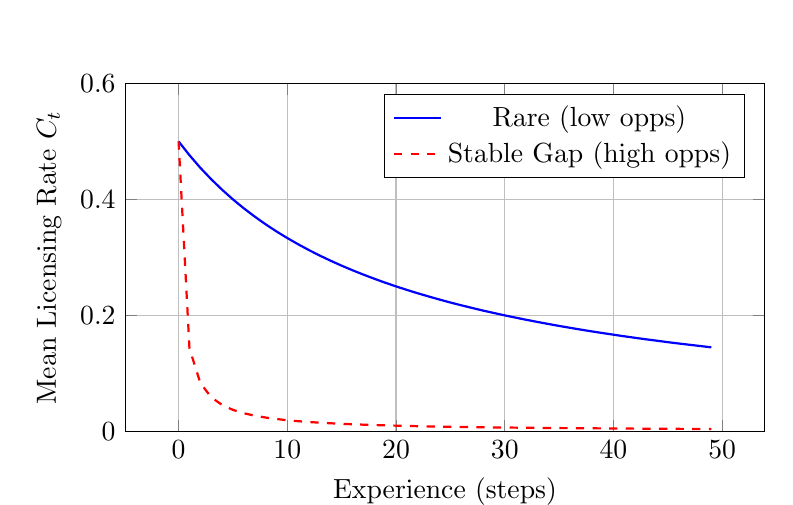
\begin{tikzpicture}
\begin{axis}[
    width=0.8\textwidth,
    height=6cm,
    xlabel={Experience (steps)},
    ylabel={Mean Licensing Rate $C_t$},
    ymin=0, ymax=0.6,
    grid=major,
    legend entries={Rare (low opps), Stable Gap (high opps)},
    legend pos=north east
]
\addplot[mark=none, blue, thick] coordinates {
(0,0.5000) (1,0.4762) (2,0.4545) (3,0.4348) (4,0.4167) (5,0.4000) (6,0.3846) (7,0.3704) (8,0.3571) (9,0.3448) (10,0.3333) (11,0.3226) (12,0.3125) (13,0.3030) (14,0.2941) (15,0.2857) (16,0.2778) (17,0.2703) (18,0.2632) (19,0.2564) (20,0.2500) (21,0.2439) (22,0.2381) (23,0.2326) (24,0.2273) (25,0.2222) (26,0.2174) (27,0.2128) (28,0.2083) (29,0.2041) (30,0.2000) (31,0.1961) (32,0.1923) (33,0.1887) (34,0.1852) (35,0.1818) (36,0.1786) (37,0.1754) (38,0.1724) (39,0.1695) (40,0.1667) (41,0.1639) (42,0.1613) (43,0.1587) (44,0.1563) (45,0.1538) (46,0.1515) (47,0.1493) (48,0.1471) (49,0.1449)
};
\addplot[mark=none, red, thick, dashed] coordinates {
(0,0.5000) (1,0.1429) (2,0.0833) (3,0.0588) (4,0.0455) (5,0.0370) (6,0.0312) (7,0.0270) (8,0.0238) (9,0.0213) (10,0.0192) (11,0.0175) (12,0.0161) (13,0.0149) (14,0.0139) (15,0.0130) (16,0.0122) (17,0.0115) (18,0.0109) (19,0.0103) (20,0.0098) (21,0.0093) (22,0.0089) (23,0.0085) (24,0.0082) (25,0.0079) (26,0.0076) (27,0.0073) (28,0.0070) (29,0.0068) (30,0.0066) (31,0.0064) (32,0.0062) (33,0.0060) (34,0.0058) (35,0.0056) (36,0.0055) (37,0.0053) (38,0.0052) (39,0.0051) (40,0.0050) (41,0.0048) (42,0.0047) (43,0.0046) (44,0.0045) (45,0.0044) (46,0.0043) (47,0.0042) (48,0.0041) (49,0.0040)
};
\end{axis}
\end{tikzpicture}
\caption{Simulation of situational licensing rate $C_t$ under preemption. When effective opportunity mass is high (Stable Gap, red), $C_t$ is driven rapidly to zero. When opportunities are rare (Situationally-Novel, blue), $C_t$ declines slowly, leaving the construction in a state of indeterminacy rather than categorical rejection.}
\label{fig:simulation}
\end{figure}

\section{Dynamics: why the state tends to become what it is}
\label{sec:dynamics-new}

The dynamics module explains trajectories of $C_t(u,c)$ (and, in principle,
refinements of the conditioning partition itself).  It doesn't define grammaticality.

\subsection{Niches, competitors, and opportunity sets}
\label{sec:niches}

Let $n$ index a \term{constructional niche} (a communicative job), and let
$\mathcal{V}_{n}$ be the set of competitor variants that can do that job
in some conditioning states.
Let $N_t(n,c)$ be the number of opportunities for niche $n$ in conditioning state $c$
over some time window, and $k_t(v,n,c)$ the observed count of variant $v\in\mathcal{V}_n$.

\subsection{Usage as \texorpdfstring{licensing $\times$ choice}{licensing x choice} among licensed options}
\label{sec:usage}

Separate \term{licensing} from \term{selection}.  A variant can be licensed but rarely chosen.

Let $\rho_t(v\mid n,c)\in[0,1]$ be the probability of choosing $v$ among those who license it
in niche $n$ under $c$.  A flexible choice model is a softmax over utilities:
$$
\rho_t(v\mid n,c)=\frac{e^{U_t(v;n,c)}}{\sum_{v'\in\mathcal{V}_n}e^{U_t(v';n,c)}},
\qquad
U_t(v;n,c)=\boldsymbol{\theta}^{\top}\mathbf{f}(v;n,c).
$$

At the population level, the expected usage rate $\pi_t(v\mid n,c)\approx C_t(v,c)\cdot \rho_t(v\mid n,c)$.



\subsection{Dynamics: preemption as effective opportunity mass}
\label{sec:update}

The core idea is that
learners update licensing not only from positive uses of $u$ but also from
structured non-occurrence when $u$ is a plausible competitor and is repeatedly
not chosen. The update shouldn't treat all \enquote{opportunities} as equally
informative: absence is evidential only to the extent that $u$ would have had
non-trivial probability of being chosen if it were licensed.

For a target variant $u$ associated with niche $n(u)$, define the \term{effective
preemption mass} in a time window as the expected number of $u$-tokens that would
have been produced if $u$ were a licensed competitor:
\begin{equation*}
p_t(u,c)
=\sum_{j=1}^{N_t(n(u),c)}
\rho_t\!\bigl(u\mid n(u),c\bigr),
\end{equation*}
where $N_t(n(u),c)$ is the number of niche opportunities observed in that window.
This quantity is large only when (i) the opportunity set is large and (ii) $u$
would have been chosen at non-trivial rates if licensed.

A simple Bayesian learner for licensing represents each $(u,c)$ with a Beta
posterior $\mathrm{Beta}(a_t,b_t)$, updated by three evidence streams:
$s_t$ (positive evidence), $e_t$ (error evidence), and $p_t$ (effective preemption mass).
Update: $a_{t+1}=a_t+s_t$, $b_{t+1}=b_t+e_t+p_t$.
The implied population mean licensing rate is then:
\begin{equation}\label{eq:beta-update}
C_{t+1}(u,c)=\frac{a_{t+1}}{a_{t+1}+b_{t+1}}.
\end{equation}

\begin{note}
\textbf{The mean-field approximation.} While I treat the discrete update \eqref{eq:beta-update} as the primary dynamics, it is sometimes useful to approximate the expected trajectory of the posterior mean $C_t(u,c)$ by a deterministic ODE. Under stationarity and large-sample assumptions, replacing the stochastic evidence streams by their expectations yields an approximation of the form $\dot{C}=r(u,c)\,C(1-C)$, where $r(u,c)$ is a net evidence rate (roughly, expected positive evidence minus expected preemption/error evidence per unit time, with $\rho_t$ determining the effective opportunity mass). I use this ODE only for qualitative fixed-point and comparative-statics arguments.
\end{note}


\subsection{How apparent categorical gaps arise without hard bans}
\label{sec:categorical-without-bans}

When $\mathsf{map}(u,c)=1$ and $K(u,c)$ is high but $C_t(u,c)$ is driven toward zero by
persistent preemption in a large opportunity set, the community converges on a sharp,
non-satiating rejection profile.  Additional processing penalties in $\mathbf{R}_i(u,c)$
(e.g.\\ systematic garden-path repair due to an entrenched fused-head construal) can strengthen
the subjective categoricality without any independent structural veto being posited.

This approach transforms the framework from a descriptive theory into a quantitative model capable of precise predictions about grammaticality judgments and their evolution over time.


% Section deleted and merged into sec:feeling-new





\section{Theoretical implications}\label{sec:implications}

MVMG yields several important implications for the understanding of grammaticality:

First, it supports treating grammaticality as an emergent property unified by the stability of form--value relations. Different patterns in the distribution of grammatical constructions across adjective types illustrate this~--  despite the existence of clear patterns governing modifier selection by adjectives, these patterns resist reduction to simple rules. Instead, they arise from complex interactions between modifier semantics, adjective scale structure, and discourse-pragmatic factors. For instance, the distribution of \textit{much} versus \textit{more} with different adjective classes (comparative governors, participial adjectives, etc.) shows complex patterns that can be explained but not easily predicted from simpler principles \autocite{reynolds2024why}. This helps explain why efforts to reduce grammaticality to simple necessary and sufficient conditions have repeatedly fallen short.

Second, this framework clarifies how formal and usage-based approaches capture different aspects of grammatical stability. The stability of grammatical patterns depends both on their internal systematic properties (emphasized by formal approaches) and on their role in meeting communicative needs (emphasized by functional accounts). Many grammatical phenomena exhibit stability patterns that can't be reduced to local collections of features. Consider how discourse context affects grammaticality judgments: whether a construction maintains stable form--value relationships often depends on broader patterns of language use that can't be localized to specific morphosyntactic features. This helps explain why purely local syntactic models often fail to capture the full range of grammaticality phenomena.

Third, the analysis suggests specific predictions about how grammatical stability is maintained and lost. If grammatical constructions are maintained through multiple interacting factors, one should expect:
\begin{enumerate}
    \item Instability to manifest in coordinated ways across multiple properties rather than through isolated changes
    \item Periods of gradually increasing instability followed by relatively rapid reorganization when stability thresholds are crossed
    \item Different but equally stable grammatical patterns emerging in different language communities
    \item Gradient effects in grammaticality judgments reflecting varying degrees of stability
\end{enumerate}

Fourth, MVMG illuminates the relationship between competence and performance. Rather than treating these as fundamentally different phenomena, they can be understood as different manifestations of the same stability conditions. Processing limitations and other performance factors help shape which form--value relations become stable, while those stable pairings in turn constrain possible performance patterns.

Finally, this approach offers a new perspective on systematic constraints in grammar, such as the English ban on left-branch extraction. Instead of viewing these as either innate rules or processing limitations, they can be understood as particularly robust stability conditions in form--value relations. Their persistence reflects deep patterns of stability, while cross-linguistic variation shows how different stable solutions can emerge in different communities.

These implications suggest concrete directions for future research. More detailed studies are needed of how multiple properties interact to create and maintain stable form--value relations, better methods for measuring degrees of stability, and closer examination of the transition points where grammatical systems reorganize. The framework also calls for renewed attention to variation across language communities, as different stability patterns may shed light on the fundamental nature of grammatical organization.

The crucial idea is that grammaticality represents a real linguistic kind~--  stable form--value relations maintained through community practice~--  rather than merely a disjunctive collection of sufficient conditions. This unifying concept helps explain both the diversity of grammatical phenomena and their underlying commonality.

\subsection{Actuation and the dynamics of grammatical change}

The concept of \textit{actuation} can now be defined as a sign change in the expected evidence balance for licensing. Informally, actuation occurs when the expected positive stream $s_t(u,c)$ begins to outweigh the combined negative streams $e_t(u,c)+p_t(u,c)$ across successive windows, so that the posterior mean $C_{t+1}(u,c)$ in \eqref{eq:beta-update} increases rather than decays. In the mean-field approximation (box in \S\ref{sec:update}), this corresponds to the regime in which the net evidence rate $r(u,c)$ becomes positive, yielding the familiar S-curve at the population level.

The factors that drive such bifurcations align with the motivations discussed in \S\ref{sec:motivations}. Semantic reanalysis may increase utility (and thus $\rho_t$) by making a form--value relation more transparent or useful. Social pressures may shift utilities (prestige effects) or alter the relevant community standard. Structural motivations such as analogical extension can systematically raise licensing probability by borrowing strength from frequent neighbors. Processing innovations may reduce error rates ($e_t$) or locality costs, improving the net evidence balance.

Actuation isn't simply a matter of individual innovation but requires coordinated community-level change. A few speakers adopting a marginal construction doesn't guarantee its success; actuation demands that the underlying dynamics shift such that acceptance systematically outweighs rejection across the speech community. This explains why many innovations fail despite being individually sensible~--  they appear before the community conditions are right for the evidence balance to become positive.

The bifurcation framework also clarifies why certain changes appear to accelerate once they begin. Near the critical point where evidence streams balance, small perturbations in community attitudes can trigger rapid shifts between rejection and acceptance. As the evidence balance becomes more strongly positive, the construction moves further from the unstable rejection state, making reversal increasingly unlikely. This creates the characteristic S-curve pattern observed in many documented language changes~\autocite{kroch1989}, emerging naturally from the underlying population dynamics.

For constructions currently existing in the marginal zone~--  those with near-zero evidence balance~--  the framework predicts heightened sensitivity to external factors and greater cross-community variation. Small speech communities may show particularly volatile behaviour near bifurcation points, as stochastic effects can overwhelm weak deterministic trends. This may explain why certain changes appear to originate in geographically or socially peripheral communities before spreading to larger population centres.

\subsection{Macro-typological constraints on grammatical design}

Recent macro-typological work sharpens the question of how strongly grammar is constrained across languages. \textcite{verkerk2025} test 191 implicational universals from the Universals Archive against Grambank’s 2{,}430-language morphosyntactic sample, using Bayesian models that control explicitly for genealogical and areal non-independence and then follow up with spatiophylogenetic analyses of evolutionary rates. A naïve analysis that ignores relatedness appears to support the vast majority of proposed universals, but once phylogeny and geography are accounted for, only about a third (60 of 191) remain statistically supported. Support is concentrated in relatively narrow domains: most hierarchical universals and a substantial minority of “narrow” word-order universals survive, whereas “broad” word-order universals and miscellaneous others fare poorly. Diachronically, supported universals typically correspond to “harmonic” combinations of features (for instance, consistent head–dependent orders) that languages are more likely to evolve into than out of, with these preferred configurations recurring independently across lineages.

From an MVMG perspective, these findings are best viewed as identifying recurrent attractors in the global design space of morphosyntactic form–value relations rather than as evidence for a small set of exceptionless grammatical laws. On the present account, such attractors correspond to configurations for which the net evidence balance (positive evidence $s_t$ vs.\ preemption/error mass $e_t+p_t$) in the entrenchment dynamics of \S\ref{sec:update} is positive across a wide range of communities: they are cognitively and communicatively favourable enough that repeated episodes of change tend to push $C_t(u,c)$ toward fixation in lineage after lineage. At the same time, the fact that roughly two-thirds of the tested universals fail once autocorrelation is controlled for dovetails with a de-idealized view of grammaticality. Community-specific conventions still have considerable freedom in how they realize form–value relations, with only some regions of the space strongly preferred. Large-scale comparative work of this kind therefore complements MVMG: it circumscribes which parts of morphosyntactic possibility space are globally stable, while the present framework provides a meso-level account of how local community dynamics and form–value coherence give rise to those long-run macro-typological regularities.

\subsection{Relationship to generative grammar}

The generative tradition has provided linguistics with foundational contributions into the systematic nature of grammatical knowledge. Most fundamentally, it demonstrates that grammaticality can't be reduced to semantic plausibility, processing ease, or frequency of attestation. When Chomsky introduced \textit{Colorless green ideas sleep furiously}, he showed definitively that speakers can recognize syntactically well-formed sentences even when they are semantically bizarre. The framework coherently explains categorical constraints like the impossibility of extracting determiner-adjective sequences in English (*\textit{Which do you prefer car?}), and critically, it captures the fact that such sequences remain ungrammatical even when their intended meaning is clear and processing demands are low. 

MVMG shares with generative grammar several foundational observations: that grammaticality judgments reflect systematic, real patterns \autocite{dennett1991}; that these patterns can't be reduced to meaning or processing alone; and that certain syntactic configurations appear to be categorically excluded regardless of context. The analysis of multiple center embeddings presented in \S\ref{sec:processing} builds directly on ideas about recursive structure, and my treatment of systematic blocking (\S\ref{sec:systematic-blocking}) acknowledges the generative discovery that some constructions appear to be universally excluded by the grammar itself.

The generative tradition has also identified fascinating puzzles that any theory of grammar needs to address, such as the independent relative \mention{whose} (\ref{ex:whose}). As \textcite{hankamer1973whose} observe, this construction appears to violate no syntactic principles: independent genitives are possible (\textit{Mine was visiting}), independent interrogative \mention{whose} is grammatical (\textit{Whose was open?}), and \mention{whose} functions perfectly well as a dependent relative pronoun (\textit{the student whose friend was visiting}). The generative tradition's careful documentation of such cases, where seemingly parallel constructions show puzzlingly different grammatical status, has been invaluable in pushing theoretical development forward.

Where MVMG departs from generative grammar is in its explanation of such patterns. Rather than positing an autonomous syntactic component, MVMG suggests that grammatical constraints emerge from the interaction of form--value relations within specific communicative situations. The independent relative \mention{whose} construction illustrates this difference. For this construction to be felicitous, multiple conditions have to converge: the possessor has to be sufficiently accessible in the discourse while the possessum is predictable enough to license ellipsis, but the possessive relationship needs to be semantically significant enough to warrant explicit marking, and this configuration has to occur in a context where a relative clause is the optimal way to package this information. The extreme rarity of contexts satisfying all these conditions appears to prevent the construction from becoming conventionalized in the grammar at all~--  speakers encounter it so rarely, despite perfectly common components, that even when all conditions align perfectly, the construction feels alien.

This approach draws on the generative observations about systematic constraints while providing a different perspective on their source. Where generative theory has to explain why a syntactically possible and pragmatically useful construction is systematically avoided, MVMG suggests that extreme mismatches between predicted and observed frequency may themselves be evidence of grammatical blocking, even when the exact nature of the block remains unclear. The framework thus preserves what is most valuable in generative theory~--  its recognition of systematic grammatical constraints~--  while embedding those insights in a broader theory of how form--value relations become established and maintained in language communities.

Other cases that generative grammar struggles to explain are those that are grammatical with one meaning but ungrammatical with another, such as (\ref{ex:have-years-sem}) \textit{I have 16 years}. While syntactically identical to grammatical expressions like \mention{I have 16 dollars}, this construction becomes ungrammatical specifically when used to express age. A purely syntactic account would have to explain why the same structure is well-formed in one case but ill-formed in another, despite no apparent syntactic differences. MVMG, in contrast, locates the source of ungrammaticality in the community's form--value conventions: \mention{have}+numeral years has become conventionalized for expressing duration or future time (\textit{I have 16 years until retirement}) but blocked for expressing age, where a different construction (\textit{I am 16 years old}) is the established pattern. Similar cases arise with plural forms that are grammatical with some meanings but not others (e.g.\, \mention{peoples} for ethnic groups but not multiple individuals) and with verbs that resist certain arguments despite no obvious syntactic prohibition (e.g.\, \mention{discuss about}). These meaning-dependent grammaticality patterns suggest that what gets blocked or licensed often depends on specific form--value associations rather than purely structural constraints.

\subsection{Relationship to Construction Grammar}

Construction Grammar (CxG) \autocite{fillmore1988mechanisms, kay1999grammatical,  goldberg1995constructions, goldberg2019, sag2012sign} represents a significant theoretical advance in the understanding of linguistic knowledge. At its core, CxG argues that language consists of learned pairings between form and meaning at multiple levels of complexity. These form--value relations, or constructions, range from individual morphemes to abstract syntactic patterns. This perspective helps explain phenomena that proved challenging for earlier approaches, which often struggled to account for how speakers learn and use both regular patterns and idiomatic expressions without requiring separate mechanisms for \enquote{core} grammar versus \enquote{periphery}.

CxG's most valuable contribution lies in demonstrating that meaning suffuses all levels of grammatical organization. Rather than treating syntax as an autonomous formal system that interfaces with semantics only at certain designated points, CxG reveals how meaning and form are inseparable aspects of linguistic knowledge. For instance, the \textit{What's} X \textit{doing} Y? construction (as in \textit{What's this fly doing in my soup?}) carries an implication of incongruity that can't be derived from its component parts \autocite{kay1999grammatical}. Such examples provide compelling evidence that constructional meaning exists beyond pure compositionality and that constructions inherently package form and meaning together.

Recent work strengthens the empirical foundation for CxG's framework. \textcite{weissweiler2023construction} demonstrate how construction grammar provides a theoretical framework for probing how neural language models handle different levels of linguistic abstraction. Their findings suggest that transformer models may learn construction-like representations, offering new evidence for CxG's cognitive reality while also providing tools for analyzing artificial neural networks.

MVMG shares these fundamental CxG views about the centrality of form--value relations and the importance of treating meaning as integral to grammar rather than merely interfacing with it. But MVMG departs from CxG on at least one key point: while CxG treats all constructions as instances of the same theoretical kind, differing only in their internal complexity and degree of schematicity, MVMG maintains that morphosyntactic form--value relations play a uniquely privileged role in grammaticality judgments.

This difference becomes clear when accounting for how speakers judge various types of linguistic violations. While CxG's unified treatment of constructions suggests no principled basis for treating different types of violations differently, speakers consistently judge morphosyntactic violations (like \ungram{\mention{Furiously sleep ideas green colorless}}) as \enquote{ungrammatical} in a qualitatively different way than they judge violations of register, politeness norms, or genre expectations. Even when morphosyntactic violations result in perfectly interpretable utterances (like \mention{I have 25 years} to express age), speakers treat them as ungrammatical in a way that differs from their reactions to pragmatically inappropriate but grammatically stable expressions.

This asymmetry suggests that morphosyntax constitutes a distinct type of linguistic knowledge~--  not because it operates autonomously from meaning (as earlier formal theories claimed), but because it represents a particular kind of form--value relation that plays a special role in defining the basic combinatorial possibilities of a language. MVMG thus preserves CxG's fundamental ideas about the inseparability of form and meaning while recognizing the unique status of morphosyntactic form--value relations in speakers' grammatical knowledge.

By maintaining this position, MVMG captures what is most valuable in the CxG approach~--  its systematic treatment of form--value relations across different levels of linguistic structure~--  while better accounting for the special status that speakers accord to morphosyntactic form--value relations in their grammaticality judgments. Rather than treating this special status as evidence for autonomous syntax (as generative approaches do), MVMG suggests it reflects the unique role that morphosyntactic patterns play in establishing the basic meaning-making resources of a language community.

\subsection{Relationship to usage-based approaches}

MVMG shares with Usage-Based approaches (UBA) \autocite{bybee2006, bybee2007frequency, bybee2010} the idea that linguistic knowledge emerges from patterns of actual language use rather than from an autonomous formal system. Both perspectives reject the notion that grammaticality can be reduced to abstract rules operating independently of meaning and context. But MVMG diverges from UBA in its treatment of the special status of morphosyntactic well-formedness, particularly in cases where frequency patterns present theoretical puzzles.

The analysis of independent relative \mention{whose}, as in \textsuperscript{?}\textit{I saw Joan, a friend of whose was visiting} is a case in point. A simple UBA account might predict that this construction's marginality stems from its low frequency. But this explanation proves insufficient: the construction isn't merely rare but dramatically rarer than one would expect given the frequency of its component parts. Independent \mention{whose} appears in interrogatives (\mention{Whose is that?}), and the relative \mention{whose} is common in dependent contexts (\mention{the student whose paper was late}). Given these frequencies, analogical extension should make the independent relative use more common than it is. The extreme rarity of independent relative \mention{whose} in corpora, despite the grammatical availability of comparable elements and contexts, marks it as more than just infrequent~--  it points to a systematic gap in form--value relations.

Where UBA would treat all linguistic patterns~--  whether phonological, morphological, syntactic, or pragmatic~--  as equally driven by usage and frequency effects, MVMG maintains that morphosyntactic patterns play a uniquely central role in grammaticality judgments. This helps explain why some extremely rare constructions remain fully grammatical (like center-embedded relatives), while other constructions that should be analogically available remain stubbornly marginal despite clear communicative potential. The framework suggests that what appears to be simple rarity may sometimes reflect deeper incompatibilities in form--value mapping that resist entrenchment even when analogical patterns would predict otherwise.

This theoretical position allows MVMG to incorporate many valuable findings from UBA~--  particularly regarding the role of frequency in entrenching constructional patterns~--  while maintaining crucial distinctions between morphosyntactic well-formedness and other types of linguistic acceptability. Cases like independent relative \mention{whose} demonstrate the need for a theory that can distinguish between patterns that are simply uncommon and those that are systematically excluded from the grammar in ways that resist frequency-based explanation.

\subsection{Relationship to logicality of language accounts}

An alternative perspective, prominent in recent formal semantics, suggests certain types of unacceptability stem from the language faculty itself possessing a deductive system that identifies and filters sentences with logically trivial meanings (tautologies or contradictions) \autocite[cf.][]{del_pinal_logicality_2019, chierchia_logic_2013, fox_economy_2000}. This \enquote{logicality of language} hypothesis attempts to explain, for example, systematic restrictions on quantifiers by arguing the unacceptable cases are \enquote{L-trivial}~--  their triviality arises solely from the meaning and configuration of logical/functional terms (like \mention{every}, \mention{some}, \mention{not}), irrespective of the open-class words (like \mention{student}, \mention{run}) \autocite{gajewski_l-triviality_2009}. A key challenge is explaining why simple tautologies or contradictions (e.g.\, \mention{It is raining and it is not raining}) are often acceptable. \textcite{del_pinal_logicality_2019} argues against \enquote{Logical Skeletons} (which assume the system ignores open-class word identity) in favour of \enquote{LF+RESCALE}, a view where the system sees standard logical forms but allows optional, context-dependent modulation of open-class terms (e.g.\, interpreting the second `raining' as `raining hard') to yield non-trivial meanings.

MVMG offers a potentially broader and more unified account. While `logicality' approaches excel at explaining restrictions tied to functional vocabulary via L-triviality, MVMG aims to cover a wider spectrum of ungrammaticality, including cases not easily reducible to logical contradiction, such as absent form--value relations (\ref{ex:nonsense}), strong deviations from conventional community forms (\ref{ex:sheeps-entrench}), or extreme, unexpected rarity (\ref{ex:whose}). By grounding grammaticality in community-specific conventions (\S\ref{sec:f-m-pair-in-community}) and allowing for gradient compatibility ($K(u,c)$) and acceptance ($C_t(u,c)$), MVMG inherently accommodates cross-linguistic variation and degrees of acceptability, aspects less central to the L-triviality filter. While LF+RESCALE provides a specific mechanism for acceptable `trivialities', MVMG suggests these might arise from more general principles of interpretation within community norms, potentially avoiding the need to posit a dedicated deductive module and specific operators like RESCALE, and offering a clearer distinction between objective grammatical status and subjective processing effects or `feelings' (§\ref{sec:feeling-new}). Thus, MVMG frames grammaticality as an emergent consequence of communicative practice rather than a direct output of logical computation within syntax.



\subsection{Relationship to relevance-theoretic accounts}

Recent work by \textcite{scottphillips2024communication} offers a fundamental observation: linguistic intuitions about acceptability arise as byproduct effects of cognitive systems for interpreting communicative acts. Just as people immediately sense when a visual stimulus violates core assumptions about physical objects (as with impossible objects), they detect when utterances violate basic presumptions about communicative efficiency. Significantly, Scott-Phillips argues that unacceptability occurs not from mere inefficiency, but from an inherent impossibility of interpreting an utterance consistently with these presumptions~--  similar to how an impossible trident (Figure~\ref{fig:impossible trident}) can't be interpreted as physically cohesive in any context.

\begin{figure}
    \centering
    \includegraphics[width=0.2\linewidth]{trident.jpg}
    \caption{Impossible trident}
    \label{fig:impossible trident}
\end{figure}

MVMG shares several key premises with this account. Both frameworks reject the need for an innate grammar faculty, locating linguistic intuitions instead within general cognitive systems. Both recognize that language emerges from communicative needs rather than autonomous syntactic principles. MVMG's emphasis on community-specific form--value relations builds directly on Scott-Phillips's arguments about how communicative pressures shape linguistic conventions.

The frameworks differ primarily in their explanatory mechanisms. Where Scott-Phillips argues that grammaticality judgments reduce to impossibilities of efficient interpretation, MVMG suggests that while communicative pressures shape which form--value relations become conventionalized, these pairings then create systematic constraints that can't be reduced to efficiency alone. For Scott-Phillips, one would have to demonstrate that (\ref{ex:tense}) contains inherent contradictions making efficient interpretation impossible. MVMG instead analyzes how the meaning of tense--aspect morphosyntax clashes with the meaning of the lexeme \textit{yesterday}. While these analyses might ultimately converge, it remains unclear why the criterion of inherent impossibility of interpretation should apply specifically to morphosyntactic violations rather than to lexical-lexical conflicts or certain phonological patterns. The scope of what constitutes an interpretive impossibility requires further theoretical development.

This difference has important empirical implications. MVMG makes relatively concrete demands: it is possible to test whether specific form--value relations are stable within a community and identify precise points of morphosyntactic--lexical conflict. The challenge for relevance-theoretic accounts, as Scott-Phillips (personal communication, Dec. 16, 2024) acknowledges, lies in establishing independent, empirically vulnerable claims about what makes efficient interpretation inherently impossible rather than merely difficult. Future work comparing specific predictions of each approach~--  particularly around how novel constructions become acceptable or unacceptable~--  could help clarify their relationship and complementary insights.

\subsection{Predictions}

This framework predicts that grammaticality judgments will vary systematically across languages depending on the degree to which morphosyntactic and lexical meanings are required to align. A prime example of this variation can be seen in the cross-linguistic treatment of gendered pronouns. In Spanish, grammatical gender permeates the morphosyntactic system, mandating concord across determinatives, adjectives, and nouns. English, in contrast, exhibits a far weaker grammaticalization of gender, primarily restricted to pronoun selection. Japanese, meanwhile, lacks grammatical gender entirely, arguably using a fundamentally different system of person reference; consequently, any notion of gender primarily operates at the lexical or pragmatic level.

These cross-linguistic differences generate specific, testable predictions within the proposed framework.  I predict that Spanish speakers will judge sentences with pronoun-antecedent gender mismatches as strongly ungrammatical, reflecting the obligatory alignment of morphosyntactic and lexical gender in the language. English speakers, though, are predicted to exhibit more gradient judgments, with mismatches perceived as moderately ungrammatical due to the weaker integration of gender into the morphosyntax. Finally, Japanese speakers are expected to show the highest tolerance for such mismatches in their equivalent referential forms, potentially judging them as pragmatically infelicitous rather than grammatically ill-formed, since grammatical gender plays no role in the language.

This paradigm can be extended beyond gender to investigate other grammatical features that exhibit cross-linguistic variation in their degree of morphosyntactic integration. Similar tests could be conducted for phenomena such as number, person, definiteness, tense, aspect, and evidentiality, providing a robust empirical foundation for understanding the interplay between morphosyntactic form, lexical meaning, and the diverse ways in which languages structure grammatical systems.

\bigskip
Another key prediction of this framework is that satiation~--  the phenomenon where repeated exposure to an ungrammatical construction leads to increased acceptability~--  should be readily inducible for many types of ungrammaticality, particularly those involving mismatches between morphosyntactic and lexical meaning or those arising from processing constraints.

For instance, consider the case of the independent relative \mention{whose}, as in \textsuperscript{?}\ungram{\mention{The packages are still here, but Nathan, whose was open, just left.}} While initially judged as ungrammatical by many English speakers, this construction might become more acceptable with repeated exposure to independent relative \mention{whose}. This is because the ungrammaticality likely stems from a combination of factors:

\begin{enumerate}
    \item Low Frequency: Independent relative \mention{whose} is extremely rare, leading to a lack of entrenchment.
    \item Processing Difficulty: The construction may pose a processing challenge in retrieving the possessum from the context.
    \item Competition with a Preferred Alternative: The more frequent and established construction with the dependent relative pronoun (\textit{whose package was open}) competes with the independent \mention{whose} form.
\end{enumerate}

This multi-factorial analysis of ungrammaticality parallels findings from acquisition research. \textcite{dressler1995} demonstrate that children's early morphological development shows similar interactions between frequency, processing constraints, and competition from established forms. Their work suggests these factors represent general principles in how form--value relations become stabilized or blocked within a community.

According to the framework, repeated exposure could lead to satiation because of:

\begin{enumerate}
    \item Increased Familiarity: Repeated encounters would increase the familiarity of the independent relative \mention{whose} construction.
    \item Reduced Processing Load: With practice, the processing difficulty associated with the construction might decrease.
    \item Weakening of the Competitor: The dominance of the alternative construction might diminish as the independent \mention{whose} form becomes more entrenched.
\end{enumerate}

The framework predicts that satiation will be more likely and more pronounced for constructions where the ungrammaticality is due to factors like low frequency, processing difficulty, or weak morphosyntactic integration, rather than a violation like that imposed by left branch extraction (e.g.\, *\mention{What did you see car?}).

\bigskip
The MVMG framework also makes specific predictions about second language acquisition. Since grammaticality judgments depend on established form--value relations within a language community, learners encountering a new language should initially perceive it as lacking meaningful structure rather than explicitly ungrammatical. While some meaning may be derived through cognates or gestures, much of the input will appear as \enquote{noise} due to the absence of shared conventions. As learners begin acquiring basic form--value correspondences, they are predicted to show heightened sensitivity to violations, marking as ungrammatical many constructions that native speakers accept. This sensitivity reflects interference from L1 form--value relations and incomplete internalization of L2 norms, both of which contribute to the gradient nature of early L2 grammaticality judgments.

Finally, as learners join the L2 speech community and internalize its form--value relations, their judgments should gradually align with those of competent speakers or signers. This trajectory differs from traditional competence-based accounts, which treat grammaticality as an all-or-nothing property. Instead, the MVMG framework predicts that learners’ judgments will initially be more gradient, reflecting partial integration into multiple linguistic systems. This gradience arises from the competing influences of L1 transfer, incomplete entrenchment of L2 norms, and reduced exposure to native-like input. This view aligns with \posscite{selinker1972} concept of \term{interlanguage}, which similarly conceptualizes L2 development as involving systematic intermediate states rather than simple progression from \enquote{incorrect} to \enquote{correct} grammar.

The prediction of initial \enquote{meaninglessness} could be tested through psycholinguistic measures, such as ERP studies tracking neural responses to unfamiliar structures or self-paced reading tasks assessing the processing of anomalous input. These methods would provide empirical evidence distinguishing the MVMG framework from traditional SLA models, which emphasize innate competence and static grammaticality judgments. Integrating these predictions with research on \term{interlanguage} development and transfer could further refine the framework’s applicability to SLA contexts.

\section{Limitations}\label{sec:limitations}

While the proposed framework offers a comprehensive account of grammaticality, integrating insights from various theoretical traditions, it's not without limitations. One potential limitation lies in the framework's reliance on the concept of \enquote{community}. Defining the boundaries of a linguistic community and determining the precise set of shared norms that govern grammaticality judgments within that community can be challenging. the framework acknowledges the fluidity and heterogeneity of language use, but further research is needed to develop more precise methods for operationalizing the notion of community and measuring its influence on grammatical stability.

The framework, in its current form, may not fully capture the complexities of stylistic variation and individual preferences. While it accounts for broad patterns of acceptability and rejection, it doesn't delve deeply into the nuances of stylistic choices that fall within the realm of grammatical acceptability. Future refinements could incorporate a more fine-grained model of stylistic variation and its interaction with core grammatical principles.

Another potential limitation concerns the framework's ability to account for purely formal constraints that seem to exist independently of meaning or communicative function. While the paper argues that many seemingly arbitrary restrictions can be explained by historical processes and the interplay of various motivations, there may be residual cases of purely formal constraints that resist explanation within the current framework. Further investigation into these cases could lead to a more complete understanding of the factors shaping grammatical systems.

%Finally, the framework's emphasis on the interaction between morphosyntactic form and lexical meaning might not fully extend to phenomena at the phonology--syntax interface. While the paper briefly touches upon the role of phonological factors, a more thorough integration of phonological constraints and their influence on grammaticality judgments would be a valuable addition.

Despite these limitations, the proposed framework provides a robust and flexible foundation for understanding the multifaceted nature of grammaticality. It offers a promising avenue for future research, and the limitations outlined here serve as points of departure for further refinement and elaboration.

%\section{Methodological Considerations for Future Research}\label{sec:Methodological-Considerations}

%The development of experimental syntax since the 2000s \autocite{sprouse2016,schutze2016} has revolutionized how we measure and understand gradient acceptability. These sophisticated methodologies allow researchers to quantify subtle differences in grammaticality judgments and track how these judgments change with exposure. The experimental approach has been particularly valuable in bridging the competence--performance divide established in early generative work, providing empirical evidence for how processing constraints interact with grammatical knowledge.

%The framework’s predictions encourage empirical investigation through corpus-based, experimental, and cross-linguistic studies. Several methodological avenues stand out:

%\begin{enumerate}
%\item \textit{Corpus analysis:} Large, balanced corpora allow researchers to track frequency patterns, stability, and emergent constructions over time. Investigating rare or marginal forms (e.g.\ the independent relative \mention{whose}) in corpora can reveal whether low frequency corresponds to genuinely unstable morphosyntactic patterns or merely a sampling gap. Comparative corpus research in multiple languages can test predictions about how community values influence grammatical distinctions.

%\item \textit{Grammaticality judgment experiments:} Controlled psycholinguistic tasks, including magnitude estimation or forced-choice paradigms, can assess subtle gradience in grammaticality judgments. By manipulating exposure and increasing familiarity with marginal forms, researchers can measure satiation effects and distinguish between stable categorical constraints and constructions that become more acceptable through repeated exposure.

%\item \textit{Processing measures:} Eye-tracking, self-paced reading, and EEG studies can identify whether some judgments arise from processing overload rather than stable grammatical constraints. If a form becomes easier to parse with practice, it suggests that processing complexity, rather than an immutable rule, lies behind initial judgments of ungrammaticality.

%\item \textit{Sociolinguistic fieldwork:} Investigations in communities with distinct dialects or multilingual practices can clarify how social and pragmatic motivations shape grammatical stability. Elicitation tasks and careful comparisons across speech communities can confirm that what counts as grammatical depends on local norms rather than universal principles.

%\item \textit{Longitudinal and historical studies:} Diachronic corpora and historical grammars can trace how marginal constructions evolve, testing predictions about which factors lead certain patterns to stabilize, which fade, and which undergo reanalysis. Tracking a community’s acceptance of previously dubious constructions over time provides direct evidence for the gradual entrenchment processes posited by the framework.
%\end{enumerate}

\section{Conclusion}

This paper proposes a novel framework for understanding grammaticality, one that moves beyond the traditional competence--performance dichotomy and embraces the dynamic interplay of form, meaning, processing constraints, and sociolinguistic factors. By conceptualizing grammaticality as an emergent property of stable form--value relations within specific language communities, the framework accounts for both the categorical and gradient aspects of grammaticality judgments. It explains why some constructions are rigidly ungrammatical, others fluctuate between marginal and acceptable, and still others evolve into stable, conventionalized patterns.

The framework's core tenets~-- that grammaticality involves conventional form--value relations, that these pairings interact with processing constraints and sociolinguistic factors, and that different types of violations arise from different mismatches between form and meaning~-- provide a principled basis for understanding a wide range of linguistic phenomena. The analysis of examples drawn from both formal syntax and experimental data has demonstrated the framework's explanatory power, illuminating challenging cases that have resisted unified explanation in previous approaches.

The framework generates testable predictions about which ungrammatical constructions might change over time and offers potential applications for language teaching, clinical linguistics, and language documentation. It predicts that grammaticality judgments will vary systematically across languages depending on the degree of alignment between morphosyntactic form and lexical meaning and that satiation effects should be more readily inducible for constructions where ungrammaticality stems from factors like low frequency, processing difficulty, or weak morphosyntactic integration rather than categorical violations.

Integrating the methodologies outlined in the previous section offers a path toward a more comprehensive understanding of how form--value relations become stable within communities, what factors promote or inhibit their entrenchment, and how cross-linguistic variation arises. Future work can refine the metrics for identifying stable form--value mappings, develop computational models to predict emergent regularities, and expand the empirical base to underrepresented languages and language contact situations.

While acknowledging the limitations of the current formulation, this paper argues that the proposed framework represents a significant step toward a more comprehensive and nuanced understanding of grammaticality. By integrating insights from generative, functional, and usage-based approaches, it offers a unified perspective that recognizes the multifaceted nature of linguistic knowledge and its grounding in both individual cognition and community practice.

Future research should focus on further refining the framework, developing more precise methods for measuring form--value stability, and investigating the complex interactions between different types of motivations (semantic, social, structural, and iconic). Cross-linguistic studies, particularly those focusing on languages with different degrees of morphosyntactic integration of features like gender, will be important for testing the framework's predictions and exploring the diverse ways in which grammatical systems can emerge and evolve.

Ultimately, the study of grammaticality offers a window into the fundamental workings of human language. By de-idealizing grammaticality and embracing its dynamic, community-relative nature, it becomes possible to gain a deeper understanding of the cognitive and social forces that shape language. This framework provides a robust foundation for such investigations, paving the way for a more integrated and comprehensive understanding of what it means for an utterance to be considered part of a language.

\newpage
\appendix

\section{Turkish vowel harmony and the morphosyntax--phonology interface}
\label{app:turkish-harmony}

Turkish illustrates a sharp distinction between \term{lexical} disharmony inside stems and
\term{allomorphic} harmony on inflectional suffixes.%
\footnote{See \autocite{Sezer1981,KabakVogel2001} for discussion of the phonology and \autocite{Arik2015} for experimental evidence on native judgments.} 
Only the latter interacts with morphosyntactic well‑formedness in the sense of the MVMG.

\textsc{Stem-internal vowels: disharmony tolerated.}
Loanwords such as \mention{doktor} `doctor' violate backness harmony, but are fully acceptable;
the language community simply memorises the form, so $C(u)=1$ and $K(u)=1$.

\ea \label{ex:doktor}
\gll doktor \\
     doctor\\
\glt `doctor' (disharmonic stem, grammatical)
\z
Because no morphosyntactic feature is left unrealised, the morphosyntax--meaning
mapping $\!M(u)\!\rightarrow\!\mu(u)$ succeeds and
\begin{equation*}
\widetilde{G}_t(u,c)=C_t(u,c)\cdot K(u,c)\cdot\mathsf{map}(u,c)=1.
\end{equation*}

\textsc{Suffixal harmony: morphosyntactic requirement.}
Inflectional morphemes are lexicalised with an underspecified vowel;
the correct allomorph has to copy \textsc{[±back]} (and, for some
suffixes, \textsc{[±round]}) from the final stem vowel.
Using the \enquote{wrong} vowel leaves part of the feature bundle unrealised,
so $K(u)=0$ and the word is ungrammatical.

\ea  \label{ex:kitap-pl}
\ea[]{\gll kitap-lar\\
          book-\textsc{pl.back}\\
      \glt `books' (harmonic, grammatical)}
\ex[*]{\gll kitap-ler\\
          book-\textsc{pl.front}\\
      \glt intended \enquote{books} (suffix harmony violation)}
\z
\z

\ea \label{ex:gul-past}
\ea[]{\gll gül-dü\\
          laugh-\textsc{pst.front.round}\\
      \glt `s/he laughed' (harmonic, grammatical)}
\ex[*]{\gll gül-du\\
          laugh-\textsc{pst.back.round}\\
      \glt intended \enquote{s/he laughed} (suffix harmony violation)}
\z
\z

\textsc{MVMG account.}
For the ill‑formed *\mention{kitap-ler} and *\mention{gül-du}:

\begin{itemize}
\item \emph{Mapping} succeeds: the plural / past node selects an exponent.
\item \emph{Compatibility} $K(u,c)=0$: the chosen allomorph fails to realise the
      \textsc{[back]} feature copied from the stem.
\item \emph{Community acceptance} $C_t(u,c)=1$: every speaker knows how plural
      and past are expressed.
\end{itemize}

Hence $G_t(u,c)=0$ and speakers judge the word as categorically wrong, not merely
odd‑sounding.  By contrast, \mention{doktor} in (\ref{ex:doktor}) keeps $K(u,c)=1$;
harmony is a phonotactic preference that affects only the phonological
well‑formedness component of $F_{i,t}(u,c)$, not grammaticality.

\textsc{Localised exceptions.}
Some derivational suffixes (e.g.~\mention{-imsi} `‑ish') are lexically
marked \enquote{disharmonic}.  The community memorises them with $C_t(u,c)=1$, so no
feature remains unrealised and $G_t(u,c)=1$ despite vowel mismatch.  Clitic
boundaries that start a fresh harmony cycle \autocite{KabakVogel2001} are
handled the same way: they satisfy the morphosyntactic mapping and leave
harmony to phonology alone.

In sum, Turkish suffix harmony errors are genuine morphosyntax--phonology
interface violations, making them \emph{ungrammatical} under MVMG, whereas
stem disharmony merely lowers phonological well‑formedness and so affects only
the listener's feeling $F_{i,t}(u,c)$.



If it could be shown that phonology alone caused feelings of ungrammaticality, that would constitute a serious challenge to this framework's central claim about the necessary involvement of morphosyntactic form--value relations in grammaticality.


\newpage
\section*{Acknowledgements}
Thanks to Peter Evans, Geoff Pullum, Muhammad Ali Khalidi, and Ryan Nefdt, Irene Kosmas, and Mostafa Hasrati for comments and suggestions. I'd like to thank Jamie Ramsden for bringing up the cases of \mention{a orange} and \olang{le hiver}. Henri Kauhanen for reviewing the formalization.

I used the large language models Claude 3.5 \& 4.5; ChatGPT o1 pro \& 5.2 pro; Gemini 3; and DeepSeek V3 in drafting and editing this paper.

\newpage
\begin{sloppypar}
\printbibliography[title=References]
\end{sloppypar}


\end{document}
